% МАЛЕНЬКИЙ ФОРМАТ. ЕСЛИ РАСПЕЧАТАТЬ С ДВУС СТОРОН, 1ый БИЛЕТ ОКАЖЕТСЯ НАПРОТИВ 2ого, 3ий НАПРОТИВ 4ого И Т.Д.


\documentclass[oneside,final,8pt,]{extreport}

\usepackage[T2A]{fontenc}
\usepackage[utf8]{inputenc}
\usepackage[russian]{babel}
\usepackage{csquotes}
\usepackage{vmargin}
\usepackage{amsmath}
\usepackage{amsfonts}
\usepackage{amssymb}
\usepackage{listings}
\usepackage{enumitem}
\usepackage{algorithm}
\usepackage{algorithmic}
\usepackage{makecell}  % для переноса строк в таблицах
\usepackage[backend=biber, style=authortitle]{biblatex}  % для ссылок на литературу
\addbibresource{references.bib}
\usepackage{nopageno}

\usepackage{hyperref}  % для ссылок и цвета цитирований
\hypersetup{
    colorlinks=true,
    linkcolor=blue,
    citecolor=magenta,
    filecolor=magenta,      
    urlcolor=cyan,
    pdftitle={Overleaf Example},
    pdfpagemode=FullScreen,
}

\usepackage{graphicx}
\usepackage{wrapfig}

\setpapersize{A2}  % чтоб буквы были меньше
\setmarginsrb{1cm}{1cm}{1cm}{1cm}{0pt}{0mm}{0pt}{0mm}
\usepackage{indentfirst}
\sloppy
\usepackage{multicol}
\usepackage{tcolorbox}
\setlength{\columnseprule}{1pt}

\DeclareGraphicsExtensions{.pdf,.png,.jpg}

% \newcommand{\todo}[1]{\textcolor{red}{#1}}
\newcommand{\todo}[1]{\colorbox{red}{#1}}


\newenvironment{proof}  % док-во теорем
    {$\blacktriangle$}  % without '$'a does not work
    {$\blacksquare$}
    
\newcommand{\mathLet}{\scalebox{1.}[1.5]{$\sqsupset$}}  % math symbol 'let'

\usepackage{fontawesome}  % to import '\faEye' -- math symbol 'eye'
% \newcommand{\maeye}{\scalebox{2.}{\faEye}}  % math symbol 'eye', very big

\newcommand*\latseye{%
       \scalebox{0.25}{\begin{pspicture}(-1,-1)(1,1)
\rput(1,-.5){\eye}
\end{pspicture}\kern1em}}

\newcommand*\latdeye{%
       \reflectbox{\scalebox{0.25}{\begin{pspicture}(-1,-1)(1,1)
\rput(1,-.5){\eye}
\end{pspicture}\kern.2em}}}

\everymath{\displaystyle}
\setlength\parindent{0pt}

% \setlength{\leftmargini}{10pt}  % чтоб отступы в итемайзах были поменьше 

\newlist{itemize2}{enumerate}{1}
\setlist[itemize2,1]{label = $\bullet$, leftmargin=0em, itemindent = 1.2em}

\renewenvironment{itemize}
{\begin{itemize2}}
{\end{itemize2}}
\begin{document}

% ------------------------- ПРЕЛЮДИЯ -----------------------------

% --- BEGIN OF PAGE ----
\newpage  
\begin{tcolorbox}[colback=white, left=0mm, right=0mm]
\begin{multicols}{4}
%---------------------0--------------------
osn 1. Предел и непрерывность функций одной и нескольких переменных. Свойства функций  непрерывных на отрезке.

osn 2. Производная и дифференциал функций одной и нескольких переменных. Достаточные условия дифференцируемости.

osn 3. Определенный интеграл, его свойства. Основная формула интегрального исчисления.

osn 4. Числовые ряды. Абсолютная и условная сходимость. Признаки сходимости: Даламбера, интегральный, Лейбница.

osn 5. Функциональные ряды. Равномерная сходимость. Признак Вейерштрасса. Непрерывность суммы  равномерно сходящегося ряда непрерывных функций.

osn 6. Криволинейный интеграл, формула Грина.

osn 7. Производная функции комплексногопеременного. Условия Коши-Римана. Аналитическая  функция.

osn 8. Степенные ряды в действительной и комплексной области. Радиус сходимости.

osn 9. Ряд Фурье по ортогональной системе функций. Неравенство Бесселя, равенство Парсеваля,  сходимость ряда Фурье.

osn 10. Прямая и плоскость, их уравнения. Взаимное расположение прямой и плоскости,  основные задачи на прямую и плоскость.

osn 11. Алгебраические линии и поверхности второго порядка, канонические уравнения,  классификация.

osn 12. Системы линейных алгебраических уравнений. Теорема Кронекера-Капелли. Общее решение системы линейных алгебраических уравнений.

osn 13. Линейный оператор в конечномерном пространстве, его матрица. Норма линейного оператора.

osn 14. Ортогональные преобразования евклидова пространства. Ортогональные матрицы и их свойства.

osn 15. Характеристический многочлен линейного оператора. Собственные числа и собственные векторы.

osn 16.Формализация понятия алгоритма. Машины Тьюринга, нормальные алгоритмы Маркова. Алгоритмическая неразрешимость. Задача останова. Задача самоприменимости.

osn 17. Понятие архитектуры ЭВМ. Принципы фон Неймана. Компоненты компьютера: процессор, оперативная память, внешние устройства. Аппарат прерываний.

osn 18. Операционные системы. Процессы, взаимодействие процессов, разделяемые ресурсы, синхронизация взаимодействующих процессов, взаимное исключение. Программирование взаимодействующих процессов с использованием средств ОС UNIX (сигналы, неименованные каналы, IPC).

osn 19. Системы программирования. Основные компоненты систем программирования, схема их функционирования. Общая схема работы компилятора. Основные методы, используемые при построении компиляторов.

osn 20. Основные принципы объектно-ориентированного программирования. Реализация этих принципов в языке С++. Примеры.

osn 21. Базы данных.Основные понятия реляционной модели данных. Реляционная алгебра. Средства языка запросов SQL.

osn 22. Виды параллельной обработки данных, их особенности. Компьютеры с общей и распределенной памятью. Производительность вычислительных систем, методы оценки и измерения.

osn 23. Основные методы обработки изображений: тональная коррекция, свёртка изображений, выделение краёв.

osn 24. Линейные обыкновенные дифференциальные уравнения и системы. Фундаментальная система решений. Определитель Вронского.

osn 25. Теоремы существования и единственности решения задачи Коши для обыкновенного дифференциального уравнения первого порядка, разрешенного относительно производной.

osn 26. Функции алгебры логики. Реализация их формулами. Совершенная дизъюнктивная нормальная форма.

osn 27. Схемы из функциональных элементов и простейшие алгоритмыих синтеза. Оценка сложности схем, получаемых по методу Шеннона.

osn 28. Вероятностное пространство. Случайные величины. Закон больших чисел в форме Чебышева.

osn 29. Квадратурные формулы прямоугольников, трапеций и парабол.

osn 30. Методы Ньютона и секущих для решения нелинейных уравнений.

osn 31. Численное решение задачи Коши для обыкновенных дифференциальных уравнений. Примеры методов Рунге-Кутта.

osn 32. Задача Коши для уравнения колебания струны. Формула Даламбера.

osn 33. Постановка краевых задач для уравнения теплопроводности.  Метод разделения переменных для решения первой краевой задачи.
\vfill\null
\columnbreak
%---------------------1--------------------

\vfill\null
\columnbreak
%---------------------2--------------------
\begingroup
    % \fontsize{36pt}{50pt}\selectfont
    % \large
    \centerline{ВНИМАНИЕ!}
    \centerline{спасибо за внимание}
    \centerline{\hfill\hrulefill\hrulefill\hfill}
    \vskip1.5cm
    \centerline{GOOSi 2.0}
    \centerline{Материалы для ГОСов 6 курса. Мяу.}
    \vskip1.5cm
    
    LaTeX-исходники этого материала вы можете найти здесь: \url{https://github.com/TheFieryLynx/GOOSi2.0}

    \bigbreak
    \bigbreak
    \bigbreak
    \bigbreak
    \bigbreak
    \rightline{Мальчик, водочки нам принеси. Мы МГУ закончили.}

    \vfill
    \centerline{По разные стороны Москвы -- XXI век}
\endgroup

\vfill\null
\columnbreak
%---------------------3--------------------

\vfill\null
\columnbreak
%---------------------
\end{multicols}
\end{tcolorbox}
% --- END OF PAGE ----

% -------------------------------------------- OSN -
\newpage
% --- BEGIN OF PAGE ----
\begin{tcolorbox}[colback=white, left=0mm, right=0mm]
\begin{multicols}{4}
%---------------------0--------------------
\nsection{OSN 1-2 Основные понятия дедуктивной верификации. Методы доказательства корректности программ.} 

Целью любой верификации программы является установление соответствия программы ее требованиям. Дедуктивная верификация устанавливает это соответствие в виде логического вывода утверждения о том, что программа соответствует требованиям. При этом доказывается соответствие программы требованиям на всех входах программы.
\paragraph{Математическая модель программы}

Переменные разделяются на три типа: входные, промежуточные и выходные.

\textbf{Входные} переменные содержат исходные входные значение и никогда не меняются во время работы программы. \textbf{Промежуточные} переменные используются для хранения промежуточных результатов в процессе вычисления. \textbf{Выходные} переменные содержат значения, вычисляемые данной программой.(входные переменные будем обозначать как x1, x2, …, промежуточные как y1, y2, …, выходные как z1, z2, …).

Каждая переменная v может принимать значения из некоторого множества Dv, которое называется \textbf{доменом} переменной.

Входной домен: Dx = Dx1  Dx2  …  Dxa; Домен программы: Dy = Dy1  Dy2  …  Dyb; Выходной домен: Dz = Dz1  Dz2  …  Dzc; 

Универсальный домен D: множество значений всех возможных переменных.

Расширенный домен Dv+: домен переменной v, дополненный специальным значением \{$\omega$\}, которое не входит в универсальный домен: $D^v_+$ = Dv $\cup$ \{$\omega$\}

\paragraph{Операторы программы}
5 видов операторов программы над множеством переменных:

Начальный оператор \textbf{START}: y $\leftarrow$  f(x). Здесь f является функцией Dx $\rightarrow$ Dy+, инициализирующей промежуточные переменные программы на основе значений ее входных переменных.

Оператор присваивания \textbf{ASSIGN}: y $\leftarrow$ g(x, y). Здесь g является функцией                 Dx X Dy $\rightarrow$ $D^y_+$, вычисляющей новые значения промежуточных переменных.

Условный оператор \textbf{TEST}: t(x, y). Здесь t является предикатом на множестве значений входных и промежуточных переменных программы.

Оператор соединения  \textbf{JOIN}.

Оператор завершения  \textbf{HALT}: z $\leftarrow$ h(x, y). Здесь h является функцией Dx X  Dy $\rightarrow$ $D^z_+$, устанавливающей значения выходных переменных программы.

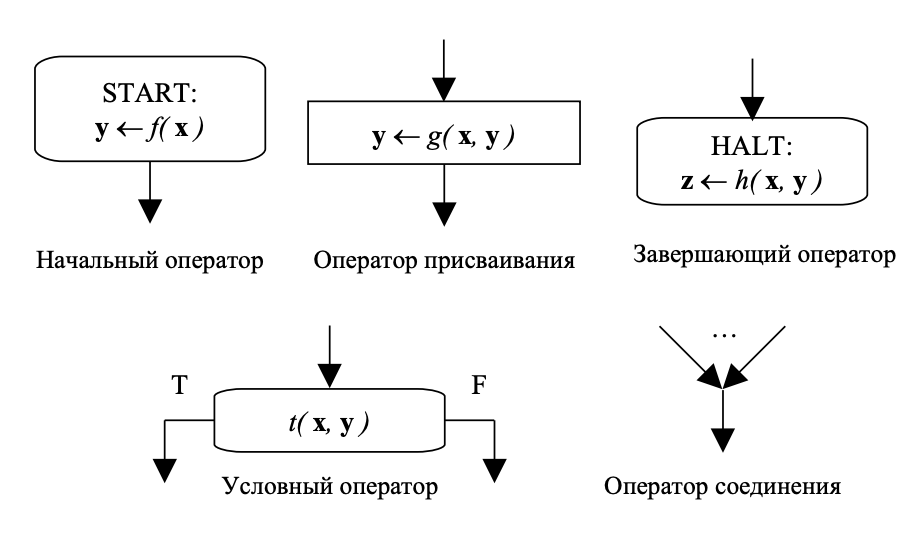
\includegraphics[scale=0.2]{pics/halt.png}

\textbf{Модель программы} - блок-схема. \textbf{Блок-схема} это тройка ( V, N, E ), где \textbf{V} – конечное множество переменных программы, \textbf{N} – конечное множество операторов блок-схемы, E $\subseteq$ N x \{ T, F, $\epsilon$ \} x N – конечное множество связок блок-схемы, помеченных символами T, F или $\epsilon$.

\textbf{Корректно-определенная блок-схема}:
\begin{enumerate}
    \item Ровно один начальный оператор и не менее одного завершающего оператора.
    \item Любой оператор находится на ориентированном пути от начального оператора к некоторому завершающему оператору.
    \item Число связок, выходящих из каждого оператора, и пометки этих связок соответствуют типу оператора: 
    \begin{itemize}
        \item Из начального оператора выходит ровно 1 дуга, помеченная символом $\epsilon$
        \item Из оператора присваивания выходит ровно 1 дуга, помеченная символом $\epsilon$.
        \item Из условного оператора выходит ровно 2 дуги, причем одна из них помечена символом T, а другая – символом F.
        \item Из оператора соединения выходит ровно 1 дуга, помеченная символом $\epsilon$.
        \item Из завершающего оператора не выходит ни одной дуги.
    \end{itemize}
    \item Число связок, входящих в каждый оператор, соответствует его типу
    \begin{itemize}
        \item В начальный оператор не входит ни одна дуга
        \item В оператор присваивания, условный и завершающий оператор входит ровно одна дуга
        \item В оператор соединения входит не менее одной дуги
    \end{itemize}
\end{enumerate}

\textbf{Определение}: $\forall$ оператора n и символа s в корректно-определенной блок-схеме (V, N, E) $\exists$ не более одного оператора n', что ( n, s, n' ) $\in$ E. Такой оператор n' (если он существует) мы будем называть \textit{последователем оператора} n по пометке s и обозначать как succ(n, s)

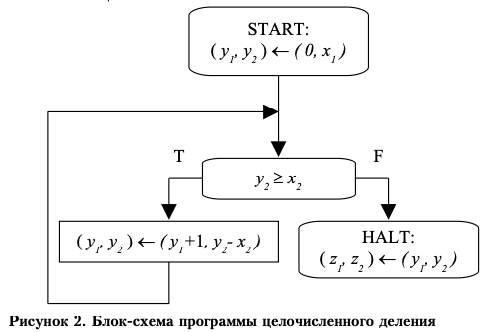
\includegraphics[scale=0.5]{pics/block_scheme.png}

\textbf{Конфигурацией программы} P будем называть пару ( \textit{l}, $\sigma$ ), где \textit{l} $\in$ $\lambda_P$ – метка текущего оператора программы, $\sigma$ =($d_1,d_2,...,d_{a+b}$ ) $\in$ $D_x^+$ x $D_y^+$ – вектор значений входных и промежуточных переменных программы.


Конечная или бесконечная последовательность конфигураций \{ $C_i$ | i=1,..,n,...\} программы P называется \textbf{вычислением}, если

\begin{enumerate}
    \item Метка первой конфигурации программы является меткой начального оператора.
    \item Значения всех входных переменных программы являются определенными ($\neq \omega$)  неизменными во всех конфигурациях вычисления.
    \item Значения промежуточных переменных в первой конфигурации равны $\omega$ (\textit{не определены}).
    \item Если метка $\textit{l}_i$ текущего оператора конфигурации $C_i$ является меткой начального оператора START: y $\leftarrow$ f(x), то следующая конфигурация $C_{i+1}$ состоит из метки оператора succ($n_i$, $\epsilon$) и вектора значений переменных $\sigma_{i+1} = \sigma_i[y \leftarrow f(x)]$.
    \item Если метка $\textit{l}_i$ текущего оператора конфигурации $C_i$ является меткой оператора присваивания ASSIGN: y $\leftarrow$ g(x, y), то следующая конфигурация $C_{i+1}$ состоит из метки оператора succ($n_i$, $\epsilon$) и вектора значений переменных $\sigma_{i+1} = \sigma_i[y \leftarrow g(x, y)]$..
    \item Если метка $\textit{l}_i$ текущего оператора конфигурации $C_i$ является меткой условного оператора TEST: t(x, y) и предикат t(x, y) при значениях переменных $\sigma_i$ принимает значение T, то следующая конфигурация $C_{i+1}$ состоит из метки оператора succ($n_i$, T) и вектора значений переменных $\sigma_{i+1} = \sigma_i$.
    \item Если метка $\textit{l}_i$ текущего оператора конфигурации $C_i$ является меткой условного оператора TEST: t(x, y) и предикат t(x, y) при значениях переменных $\sigma_i$ принимает значение F, то следующая конфигурация $C_{i+1}$ состоит из метки оператора succ($n_i$, F) и вектора значений переменных $\sigma_{i+1} = \sigma_i$.
    \item Если метка $\textit{l}_i$ текущего оператора конфигурации $C_i$ является меткой оператора соединения JOIN, то следующая конфигурация $C_{i+1}$ состоит из метки оператора succ($n_i$, $\epsilon$) и вектора значений переменных $\sigma_{i+1} = \sigma_i$.
    \item Если метка $\textit{l}_i$ текущего оператора конфигурации $C_i$ является меткой завершающего оператора HALT: z $\leftarrow$ h(x, y), то $C_i$ является последней конфигурацией вычисления.
    \item Если в конфигурации $C_{i+1}$ значение какой-либо промежуточной переменной равно $\omega$, то это последняя конфигурация вычисления.
\end{enumerate}

\textbf{Лемма}: Для каждой блок-схемы P и вектора значений ее входных переменных x существует единственное вычисление, в первой конфигурации которого значения входных переменных равны x.


\vfill\null
\columnbreak
%---------------------1--------------------
\subsection{OSN 3 Основные сведения об объектном языке ограничений (OCL): состав OCL-выражения,навигация по ассоциациям, виды коллекций, операции с коллекциями, учёт наследования в выражениях и наследование ограничений. Примеры использования OCL.}

\vfill\null
\columnbreak
%---------------------2--------------------
\nsection{OSN 5 Образцы (паттерны) проектирования, их классификация и способ описания. Примеры образцов: структурного, поведенческого и порождающего.}

Образец (или паттерн) – это типовое проектное решение конкретной задачи проектирования, описанное специальным образом, чтобы облегчить его повторное применение. Фактически, каждый паттерн является формализованным опытом лучших разработчиков в индустрии создания ПО. Основные составляющие части описания образца: Имя. Идентифицирует образец. Хорошее имя характеризует решаемую проблему и способ ее решения. Задача. Описание ситуации, в которой следует применять образец. Это описание включает в себя: постановку проблемы, контекст проблемы, перечень условий, при выполнении которых имеет смысл применять образец. Решение. Описание элементов архитектуры, связей между ними, функций каждого элемента. Включает в себя UML-диаграммы. Результаты. Следствия применения паттерна и компромиссы. Преимущества и недостатки образца. Влияние использования образца на гибкость, расширяемость и переносимость системы. 3 типа: порождающие образцы (способы создания экземпляров классов); структурные образцы (способы задания статических связей между проектными классами); образцы поведения (способы организации взаимодействий между объектами).

\textbf{Мост (Bridge) Классификация: структурный образец.}
Назначение: отделить абстракцию от реализации.
Мотивация: наследование жестко привязывает реализацию к абстракции, поэтому лучше иметь иерархию наследования для интерфейсов и отдельно их реализации.
Пример: Пусть есть абстракция Shape (форма), в ней есть операция draw(), отвечающая за отрисовку. В каждой конкретной форме (Rectangle, Circle) отрисовка реализуется с помощью примитивов drawLine(), drawCircle(), описанных в интерфейсе Drawing, реализуемом разными графическими утилитами DrawingV1, DrawingV2, рассчитанными на работу с разными графическими устройствами Driver1, Driver2. Диаграмма классов:
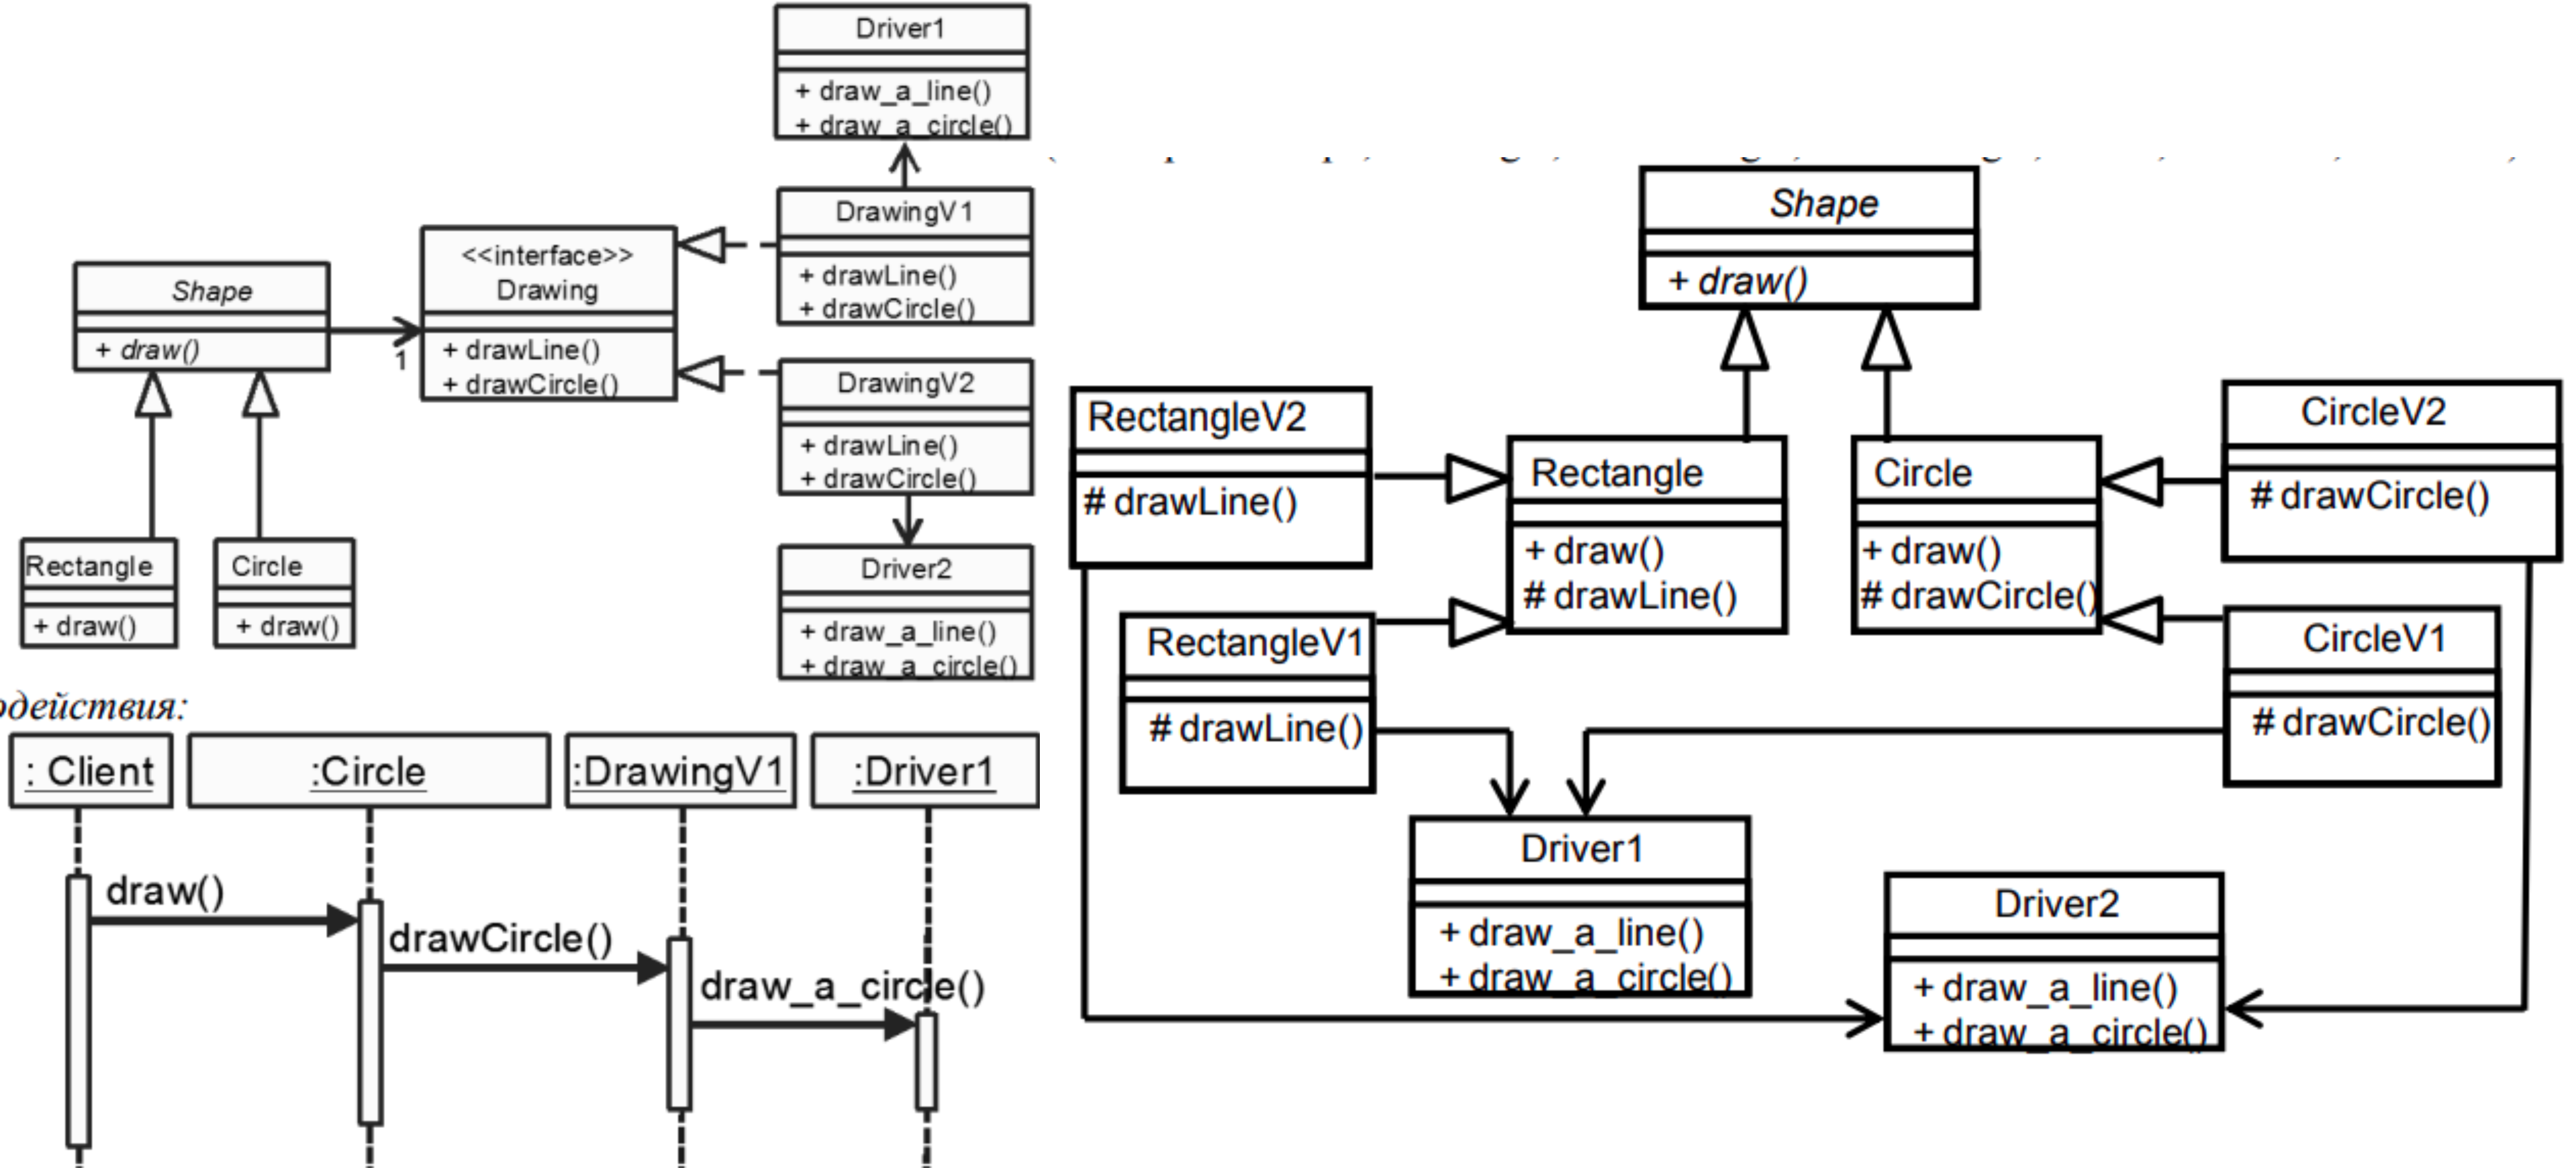
\includegraphics[scale=0.055]{pics/5_1.png}
Если не применять образец, то у Rectangle и Circle могли бы быть два наследника, каждый из которых рассчитан на работу с одним из двух вариантов графики. Т. е. в иерархии форм было бы 7 классов (см на рис.: Shape, Rectangle, V1Rectangle, V2Rectangle, Circle, V1Circle, V2Circle).Если добавить ещё формы – наследницы Shape – Triangle, PolyLine, то в первом случае при их отрисовке дополнительные классы не нужны, так как можно воспользоваться реализациями Drawing. Во втором случае иерархия разрастается, в ней становится 13 классов (добавляются Triangle, TriangleV1, TriangleV2, PolyLine, PolyLineV1, PolyLineV2). Аналогично применение паттерна Мост выгодно при добавлении поддержки еще одного графического устройства Driver3. Будет достаточно добавить новую реализацию интерфейса Drawing – класс DrawingV3, вместо того, чтобы заводить каждой конкретной фигуре наследника с реализацией отрисовки для нового устройства (RectangleV3, CircleV3, TriangleV3, PolyLineV3).

\textbf{Strategy (Стратегия) Классификация: образец поведения.} Назначение: Определяет семейство алгоритмов, инкапсулирует каждый из них и делает их взаимозаменяемыми. Мотивация: есть несколько алгоритмов решения одной задачи, которые нежелательно «зашивать» в клиентский класс. Результаты: 1 Иерархия классов стратегий определяет семейство алгоритмов или поведений, которые можно повторно использовать. 2 Инкапсуляция алгоритма в отдельный класс позволяет изменять его независимо от контекста. 3 Избавляемся от if и switch (улучшаем читаемость кода). Приведем пример использования образца для реализации разных стратегий расчета налогов:

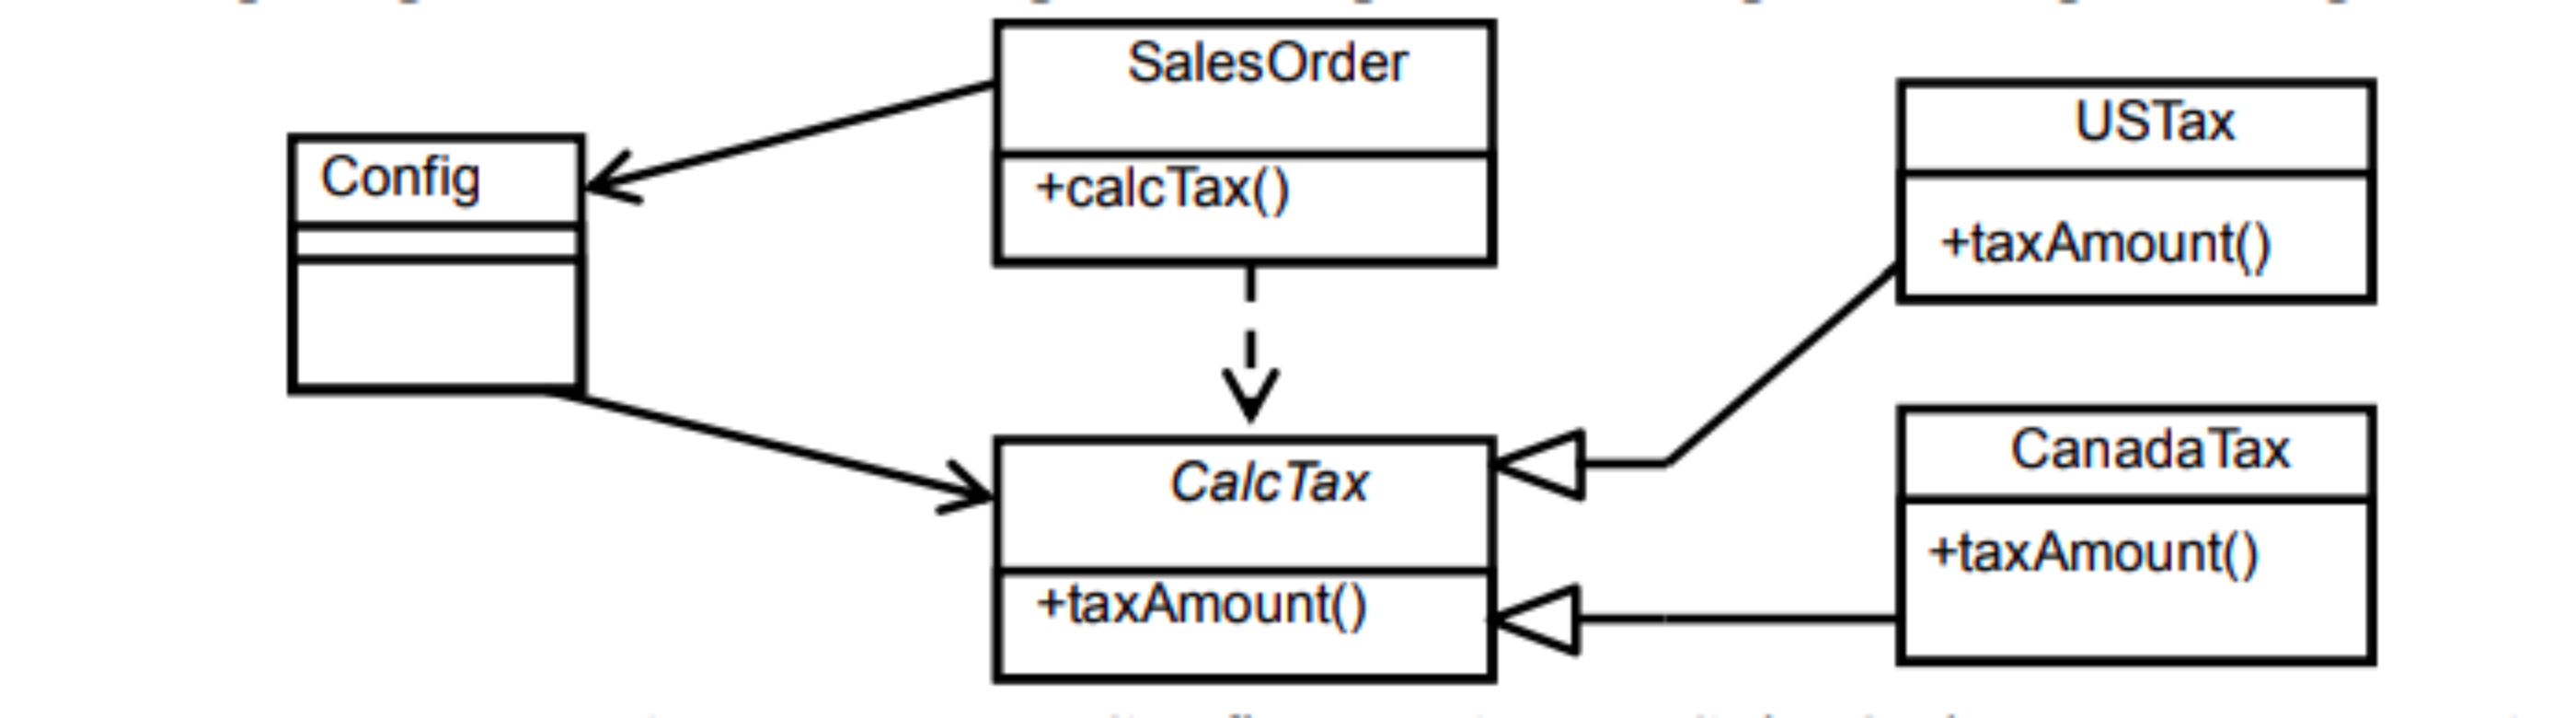
\includegraphics[scale=0.07]{pics/5_2.png}

Предполагается, что объект класса Config сообщает SalesOrder ссылку на объект-алгоритм расчета налогов (либо экземпляр USTax, пригодный для США, либо CanTax, пригодный для Канады). Если потребуется добавить новые способы расчета, достаточно добавить подклассы CalcTax. Обратите внимание, что в примере вместо интерфейса и реализации используется абстрактный класс и связи обобщения. Альтернативой предложенному решению является внесение внутрь SalesOrder::calcTax() логики выбора схемы расчета и реализация расчетов в отдельных операциях SalesOrder. Модифицируемость такого решения ниже, чем при использовании образца.

\textbf{Абстрактная фабрика (Abstract Factory) Классификация: образец порождения объектов.} Назначение: предоставляет интерфейс для создания взаимосвязанных и взаимозависимых объектов, не определяя их конкретных классов. Мотивация: часто встает задача проектирования программной системы независимой от конкретной реализации GUI. Результаты:
1 изоляция клиента от деталей реализации классов-продуктов (их имена известны только конкретной фабрике); 2 упрощение замены семейств продуктов; 3 набор классов-продуктов фиксирован, добавлять новые продукты в семейства трудно. Представим, что нужно добавить третий класс продуктов. Потребуется добавить иерархию из 3-х классов и дополнительный метод в каждую фабрику, что довольно затратно. Пример: две фабрики обеспечивают производство семейств классов-драйверов, работающих с низким или высоким разрешением. Предполагается, что разрешение драйвера принтера должно соответствовать дисплейному.

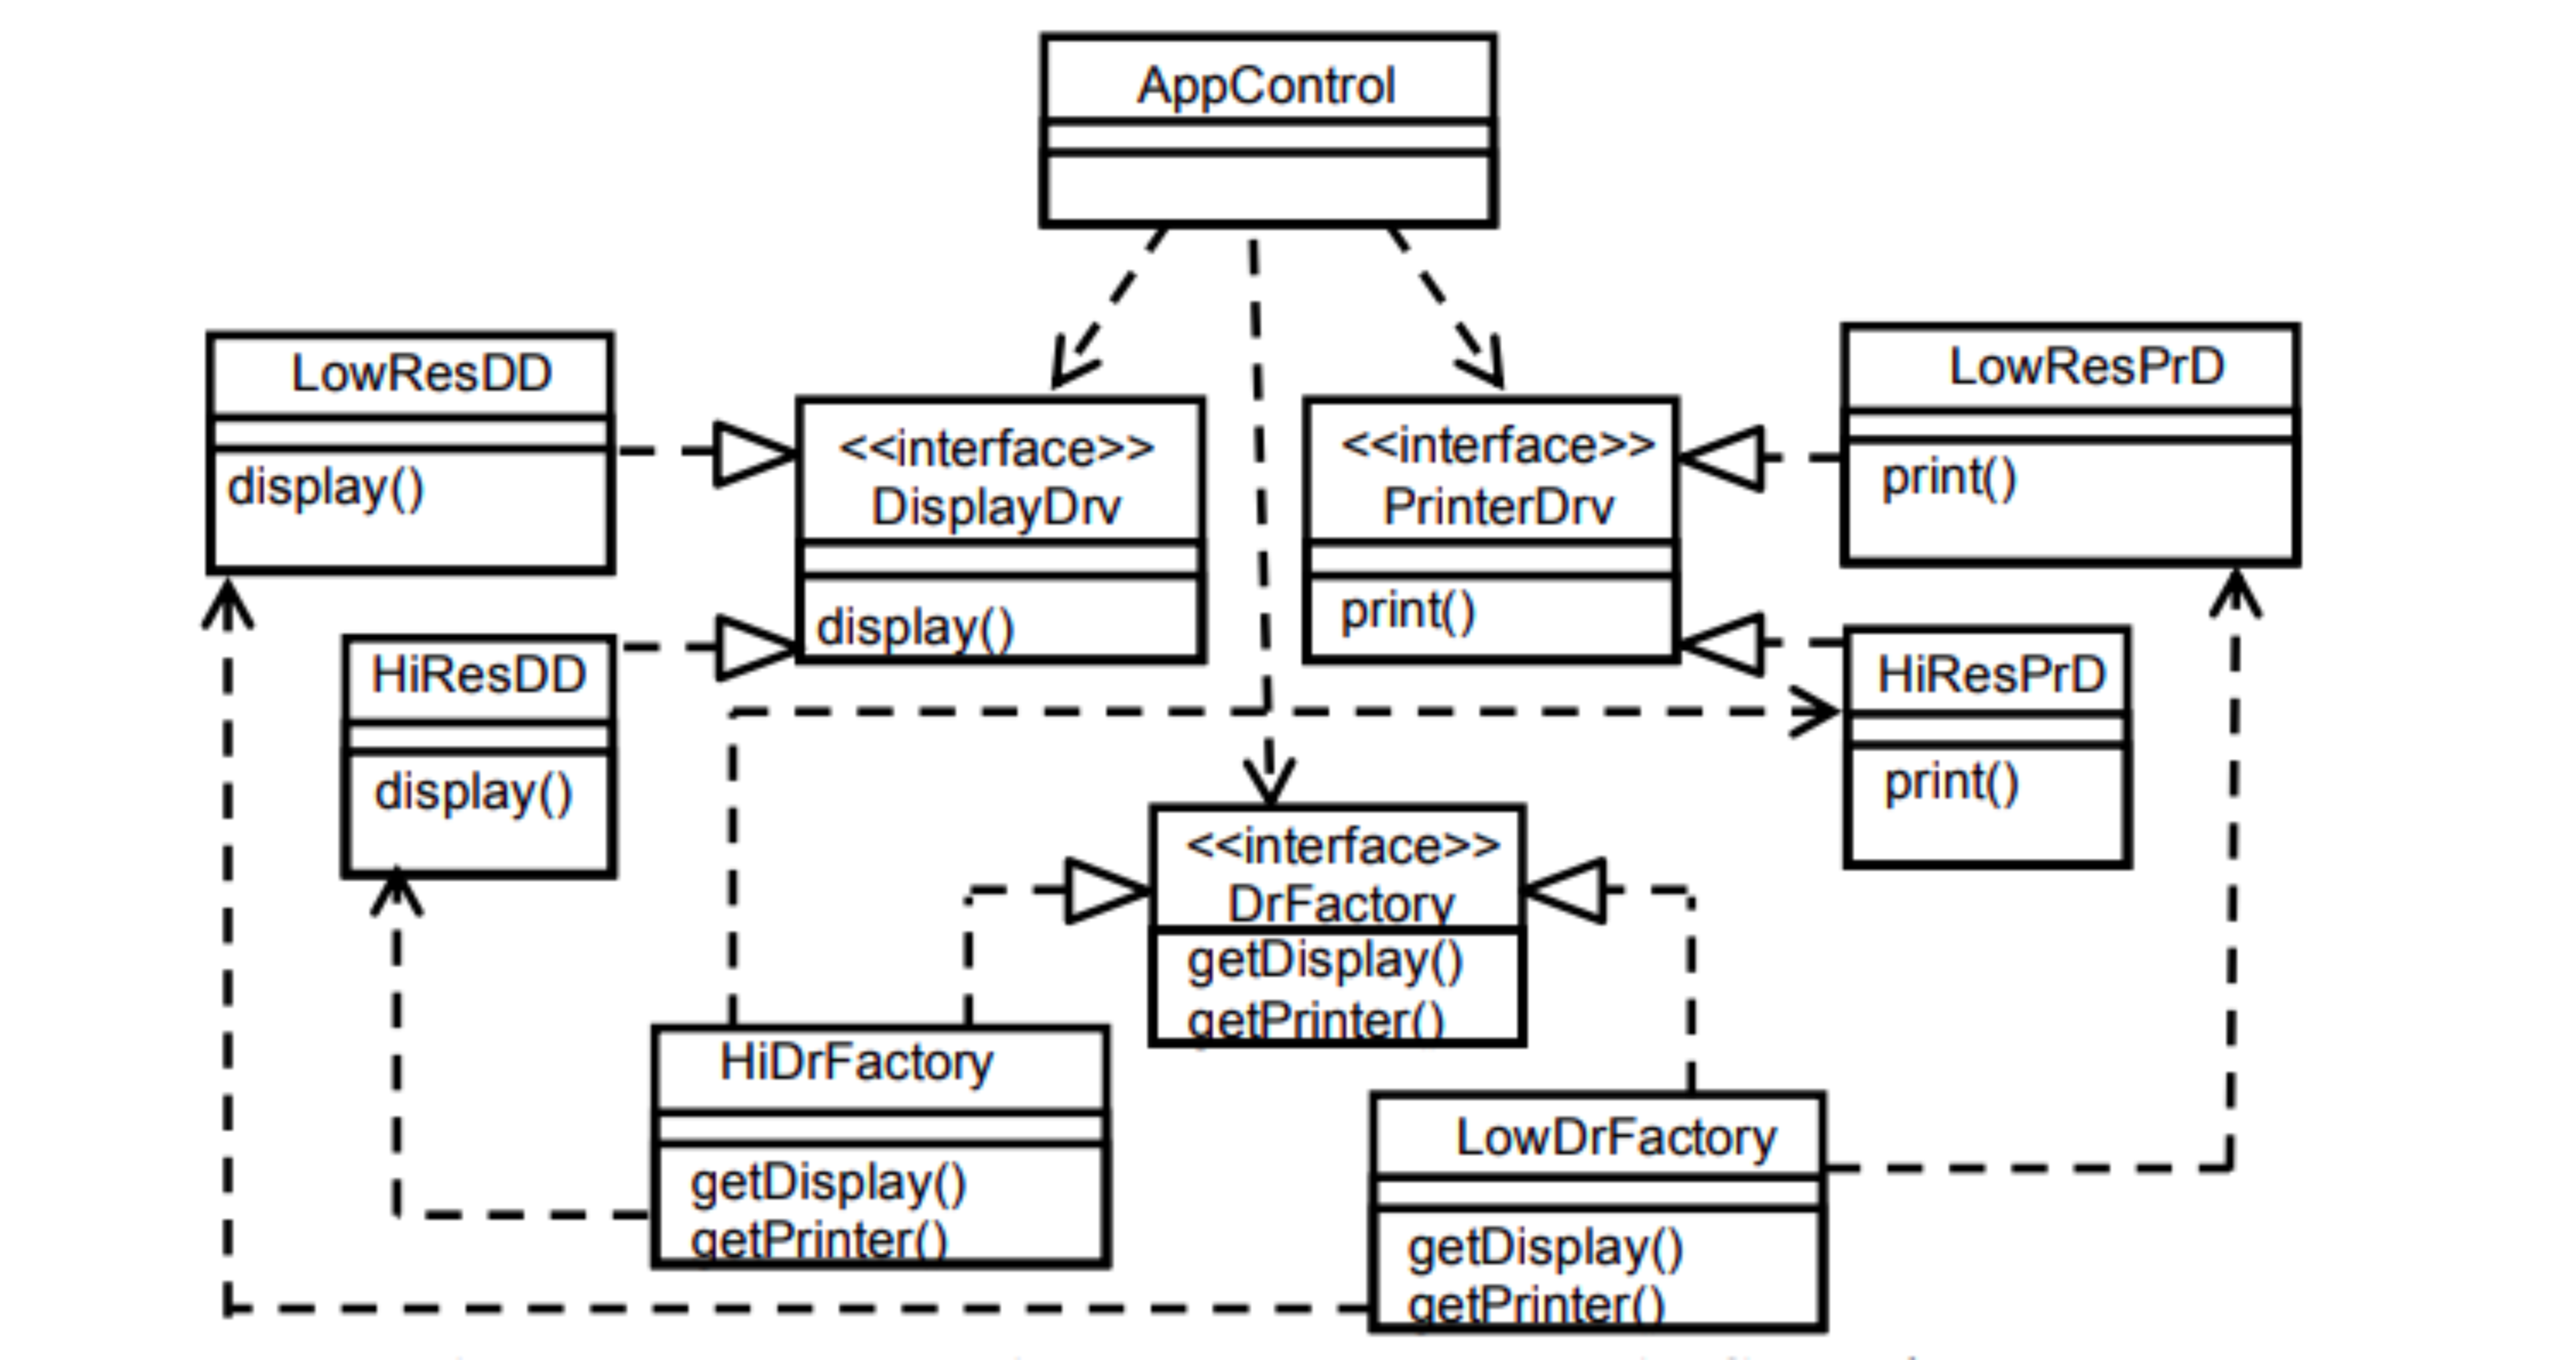
\includegraphics[scale=0.08]{pics/5_3.png}

Без применения образца пришлось бы связывать класс ApControl прямыми зависимостями с классами LowResDD, HiResDD, LowResPrD, HiResPrD. На диаграмме, приведённой выше, предполагается, что классы LowResPrD и HiResPrD могут иметь общий интерфейс (или общий суперкласс).
\vfill\null
\columnbreak
%---------------------3--------------------
\nsection{OSN 7 Ошибка типа «переполнение буфера». Выполнение произвольного кода на исполнимом стеке. Противодействие выполнению кода на стеке: «канарейка»,
DEP. Выполнение произвольного кода на неисполнимом стеке. Return-to-libc, return-orientedprogramming(ROP).}

\textbf{Ошибка типа «переполнение буфера»}
Программа осуществляет запись в буфер, размещенный на стеке, по неверному индексу, превышающему наибольший допустимый. Ошибка типична для языков Си и Си++, а также для ассемблера. Возможные последствия эксплуатации уязвимости: нарушение доступности — аварийное завершение или зависание программы; нарушение конфиденциальности, целостности и доступности — перехват потока управления, внедрение произвольного кода. CWE оценивает вероятность эксплуатации как очень высокую.

\textbf{Условия реализации атаки}
\begin{itemize}
    \item \textbf{Исполнимый стек:} внедряемый код размещён на стеке. Если система не позволяет выполнять код из диапазона адресов, относящегося к стеку, атака не удастся.
    \item \textbf{Относительно корректное завершение функции:} после того, как перезаписан адрес возврата и предшествующие ему значения в стеке, функция должна доработать до команды ret, чтобы выполнился внедряемый код.
    \item \textbf{Постоянные адреса: }в рамках последовательных запусков программы адреса объектов в стеке не должны меняться, т.к. иначе перезаписанный адрес возврата перестанет быть корректным, и вместо перехвата потока управления можно будет получить лишь аварийное завершение программы.
\end{itemize}

\textbf{Противодействие выполнению кода на стеке}

\textbf{Неисполнимый стек} (DEP) — технология, позволяющая помечать сегменты или страницы памяти стека как неисполняемые. При попытке передать управление на код, размещённый в такой памяти, происходит аварийное завершение процесса. Аппаратно поддерживается на уровне страничной трансляции во всех процессорах x86\_64, а также в более новых x86 и ARM. В более старых моделях x86 возможна более медленная и сопряжённая с дополнительными ограничениями на исполнимые файлы реализация с использованием сегментной трансляции.

\textbf{Канарейка }
Общая идея: проверять факт перезаписи стека непосредственно перед адресом возврата перед выходом из функции. «Канарейка» — как правило случайное значение, которое размещается на стеке перед адресом возврата. Перед выходом из функции происходит сравнение значения в стеке с исходным значением. Если значения не совпадают, программа аварийно завершается.

\textbf{Обход «канарейки» на стеке:}
\begin{enumerate}
    \item «Канарейка» проверяется только перед выходом из функции, однако перехват потока управления может быть осуществлён раньше (перезаписываемый указатель на функцию).
    \item «Канарейка» может быть перезаписана, если в функции есть ошибка CWE-123 (‘Write-what-where Condition’). Также в этом случае может быть перезаписан адрес возврата, а «канарейка» останется неизменной.
    \item Если программа содержит, например, ошибку CWE-126 (‘Buffer Over-read’), или возможны множественные попытки (brute force), то значение «канарейки» может быть извлечено из стека, после чего возможна эксплуатация переполнения буфера с известным значением «канарейки».
    \item Перехват обработчика исключения на Windows (SEH-эксплоит).
\end{enumerate}

\textbf{Обход DEP: return-to-libc}
 
Вместо передачи управления на код внутри буфера можно заменить адрес возврата на адрес известной библиотечной функции, например system из стандартной библиотеки Си. 

\textbf{Противодействие:}
\begin{enumerate}


    \item \textbf{Рандомизация адресного пространства (ASLR)} — изменение карты памяти процесса при каждом запуске (процесса или системы). Без дополнительных действий (PIE) адрес загрузки основного исполняемого файла не рандомизируется. Можно попытаться обойти защиту, используя только постоянные адреса.
    \item  \textbf{Return-oriented programming (ROP)}. \textbf{Гаджет} — последовательность команд в исполняемых секциях программы, заканчивающаяся командой RET. Возвратно-ориентированное программирование (ROP) — способ построения эксплоита, при котором полезная нагрузка формируется в виде цепочки гаджетов с известными постоянными адресами. 
\end{enumerate}
\vfill\null
\columnbreak
%---------------------
\end{multicols}
\end{tcolorbox}
% --- END OF PAGE ----



% --- BEGIN OF PAGE ----
\newpage  
\begin{tcolorbox}[colback=white, left=0mm, right=0mm]
\begin{multicols}{4}
%---------------------0--------------------
\nsection{OSN 8 Статический анализ исходного кода с целью поиска ошибок. Типы обнаруживаемых ошибок. Путь распространения ошибки: source, propagation, sink. Потоковая и контекстная чувствительность. Качество результата анализа: false/truepositive/negative. Интерпретация результатов анализа.}

\textbf{Анализ программы} — выявление фактов о программе;

\textbf{Статический анализ} — анализ программы без её запуска;

\textbf{Поиск ошибок} (FindBugs, Coverity, Klocwork, Svace).

\begin{itemize}
    \item \textbf{Неформальный подход} — поиск часто встречающихся ошибок:
    \begin{itemize}
        \item перекрёстная проверка кода:
        \begin{itemize}
            \item выполняется вручную;
            \item у людей похожие «слепые пятна» при просмотре кода;
        \end{itemize}
        \item анализ на уровне синтаксиса — автоматический поиск ошибочных шаблонов в коде.
    \end{itemize}
    \item \textbf{Формальный подход} — поиск всех ошибок или доказательство их отсутствия:
    \begin{itemize}
        \item верификация — формальное доказательство соответствия программы её спецификации:
        \begin{itemize}
            \item требует построения спецификации;
        \end{itemize}
        \item проверка свойств — например, <<программа не выбрасывает NullPointerException>>.
    \end{itemize}
\end{itemize}

\textbf{Ошибки работы с ресурсами:}
\begin{itemize}
    \item утечки памяти или других ресурсов;
    \item  неверная последовательность операций (например, двойное освобождение);
    \item ошибки при работе с многопоточными примитивами.
\end{itemize}

\textbf{Ошибки ввода/вывода:}
\begin{itemize}
    \item форматная строка.
\end{itemize}

\textbf{Арифметические ошибки:}
\begin{itemize}
    \item деление на ноль.
\end{itemize}

\textbf{Использование неинициализированных значений.}

\textbf{Ошибки работы с памятью:}
\begin{itemize}
    \item разыменование нулевого указателя;
    \item выход за границы буфера.
\end{itemize}

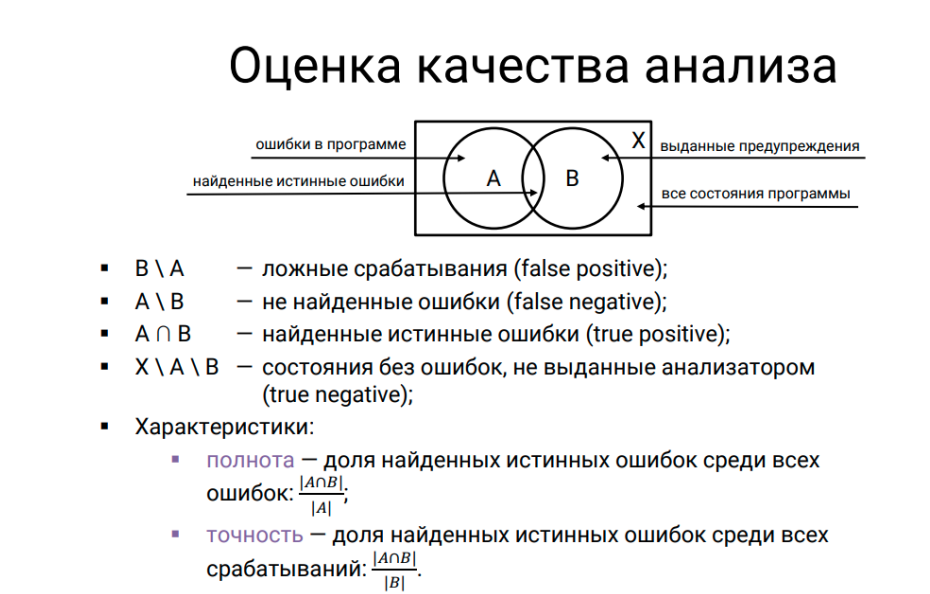
\includegraphics[width=\linewidth]{pics/quality_check.png}

\textbf{Чувствительность к пути} — способность анализа различать разные пути в программе.

\textbf{Чувствительность к потоку} — способность анализа различать порядок следования операторов.

\textbf{Чувствительность к контексту} — способность анализа различать разные вызовы одной функции.

\begin{itemize}
    \item \textbf{Цель обнаружения ошибки} — её устранение.
    \item Ошибка обнаруживается в месте её проявления в программе (выполнение некорректного действия).
    \item Исправление может требоваться в другом месте.
    \item \textbf{Путь распространения ошибки} — поток данных в программе, приведший к ошибке, делится на 3 части:
    \begin{itemize}
        \item[*] \textbf{источник (source)} — место инициализации переменных, значения которых привели к ошибке;
        \item[*] \textbf{распространение (propagation)} — операторы, участвовавшие в обработке/передаче значений, которые привели к ошибке;
        \item[*] \textbf{сток}, место проявления ошибки (sink) — оператор, приводящий к ошибке.
    \end{itemize}
\end{itemize}
\vfill\null
\columnbreak
%---------------------1--------------------
\subsection{OSN 6 Основные понятия безопасности информации: конфиденциальность, целостность,доступность. Виды защиты информации. Модель Белла-Лападулы. Понятие ошибки, уязвимости в программном обеспечении, примеры.}

\vfill\null
\columnbreak
%---------------------2--------------------
\nsection{OSN 4 Способы объектно-реляционного отображения для классов и атрибутов, бинарных и N-арных ассоциаций, классов ассоциаций, иерархий наследования. Примеры применения этих способов. Моделирование схемы реляционной базы данных с помощью диаграммы классов.}

\textbf{Реляционная} схема данных и объектная модель оперируют разными понятиями, из-за чего необходима специальная работа по объектно-реляционному отображению. Отображение возможно в обе стороны: в \textbf{прямую} (от классов к таблицам) и в обратную (от таблиц к классам). Отображение может быть таким, что для конкретной модели классов строится соответствующая только этой модели схема реляционной базы данных. Такой подход назовём зависимым от модели. Альтернативный подход – \textit{универсальный} – отличается тем, что схема реляционной базы данных подходит для любой исходной модели классов.

В качестве универсального рассматривается мэппинг Амблера, хорош универсальностью: схема не изменится (в отличие от ORM далее), если в исходную модель классов, преобразовываемую в реляционную схему, добавить/удалить класс или связь. Недостаток мэппинга Амблера в том, что операции с экземплярами, со связями, со значениями громоздки (применим только для малых моделей). Так при создании объекта нужно определить набор атрибутов его класса, создать слоты для хранения значений атрибутов в объекте. 
Переводить модель классов в схему БД предлагается в 3 этапа: отобразить классы в таблицы, отобразить ассоциации и отобразить связи обобщения. 

\textbf{ORM-стратегии классов:}

\textbf{1.} Каждый класс переводится в отдельную таблицу, столбцы которой служат для хранения значений
скалярных атрибутов, и каждая запись которой соответствует экземпляру класса. 

\textbf{2.} Уникальный идентификатор устойчивого класса (совокупность атрибутов класса, помеченных ограничением {id}) превращается в первичный ключ таблицы. Если явного идент-ра нет, то он добавляется.

\textbf{ORM-стратегии атрибутов:} 

\textbf{1.} Атрибут мощностью 1 или 0..1 (со значением скалярного типа) может быть переведён в один столбец таблицы класса. В зависимости от практических соображений один атрибут может быть переведён в несколько столбцов. Например, вместо того, чтобы хранить адрес клиента в одном столбце, можно разбить адрес на части (город, улица, дом, № квартиры и т. п.) и хранить каждую часть в отдельном столбце. \textbf{2.} Для атрибутов мощностью * заводится отдельная таблица, каждая запись которой хранит значение атрибута и ссылку (во внешнем ключе) на запись об экземпляре класса, к которому относится значение. 

\textbf{3.} Для атрибутов с точной верхней границей мощности можно не заводить отдельную таблицу, а добавить несколько столбцов (адрес1, адрес2, адрес3, …). 

\textbf{4.} Для выводимых атрибутов можно не заводить столбцов. Их значения можно не хранить, а вычислять. 

\textbf{5.} Значения статических атрибутов следует хранить в отдельной служебной таблице. Таблица для статических атрибутов может иметь несколько строк и 4 столбца: \textbf{<}id, имяКласса, имяАтрибута, значение\textbf{>}. На основе этого решения можно получить таблицу для статических атрибутов с мощностью *.

При отображении ассоциаций можно пытаться экономить и не создавать дополнительные таблицы для хранения соединений между устойчивыми объектами за счет объединения нескольких таблиц в одну или за счёт добавления внешних ключей в таблицы. \textbf{Стратегии ORM бинарных ассоциаций:} 

\textbf{1.}«1 к 1му» – возможны различные решения, лучше создать общую таблицу для 2х классов. Столбцы – совокупность атрибутов. Пример: класс <<Персона>>1<--->1<<Свид-во о рождении>>; 

\textbf{2.} «1 к 0..1» – внешний ключ добавляется к таблице необязательного класса. Вообще говоря, можно было бы использовать тот же прием, что и в «1 к 1», но получающаяся таблица будет «разреженной» – в некоторых записях будут пустые поля. Пример: класс <<Персона>>1<--->0..1<<Паспорт>> (не у всех есть паспорт) В <<Паспорт>> добавляется внешний ключ idПерсоны. 

\textbf{3.} «0..1 к 0..1» – работают оба выше указанных решения, с поправкой на изменившуюся мощность, но также рекомендуется ещё одно – отдельная таблица для связи. Пример: <<Автомобиль>>0..1<--->0..1<<Прицеп>> 

\textbf{4.} «* к *» – для ассоциации заводится отдельная таблица. Ее столбцы – внешние ключи для таблиц классов, связанных ассоциацией. Основной ключ – набор из обоих столбцов.

\textbf{ORM N-арной ассоциации:} Требуется служебная таблица для хранения связи. Например, в случае тернарной (N=3) ассоциации служебная таблица состоять из внешних ключей для каждой из трёх таблиц, полученных при ORM классов, а все её столбцы в наборе дадут её первичный ключ.

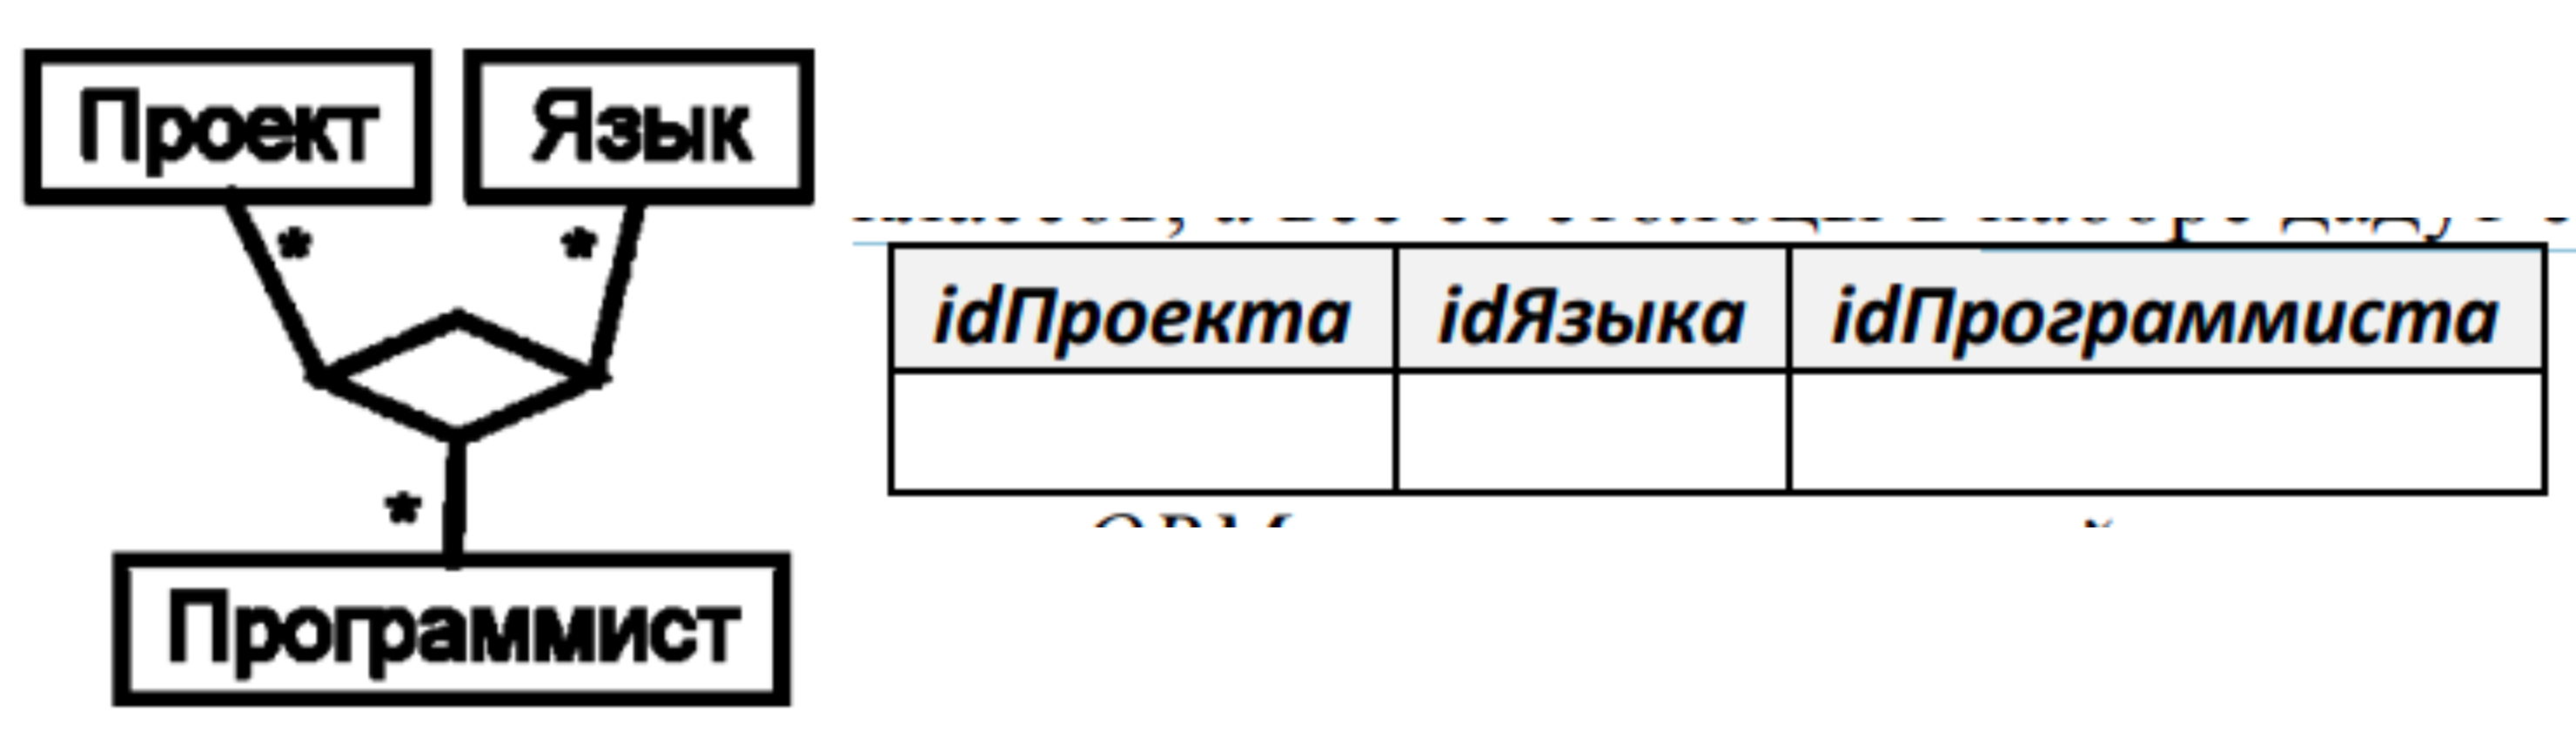
\includegraphics[scale=0.05]{pics/4_1.png}

\textbf{ORM классов-ассоциаций:} Атрибуты класса-ассоциации добавляются либо в создаваемую для связи таблицу, либо (если дополнительная таблица не требуется) в ту таблицу, куда добавляется внешний ключ, либо в общую таблицу (при слиянии).

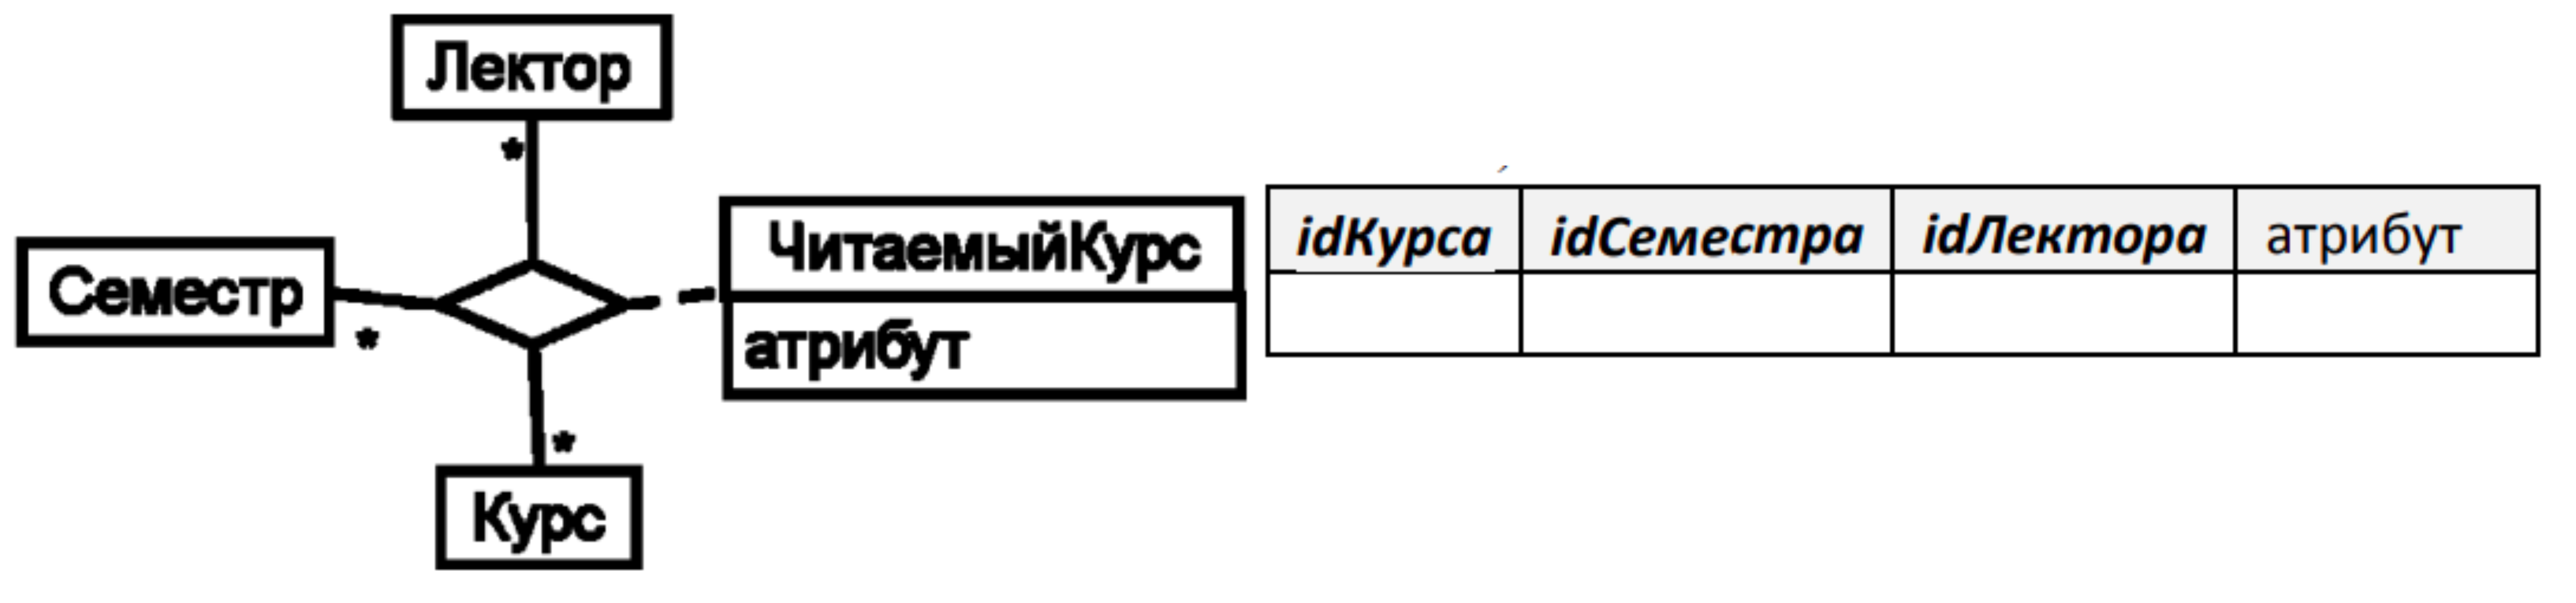
\includegraphics[scale=0.05]{pics/4_2.png}

Подводя итог ORM ассоциаций, перечислим использованные выше стратегии: слияние таблиц, добавление внешнего ключа, отдельная таблица для связи.

\textbf{ORM обобщения (наследования):}
Какой именно способ выбрать диктуют соображения эффективности (скорость в обмен на объем памяти). Рассмотрим на примере. Заметим, что класс Person – абстрактный, а класс StudentEmployee имеет двух предков.
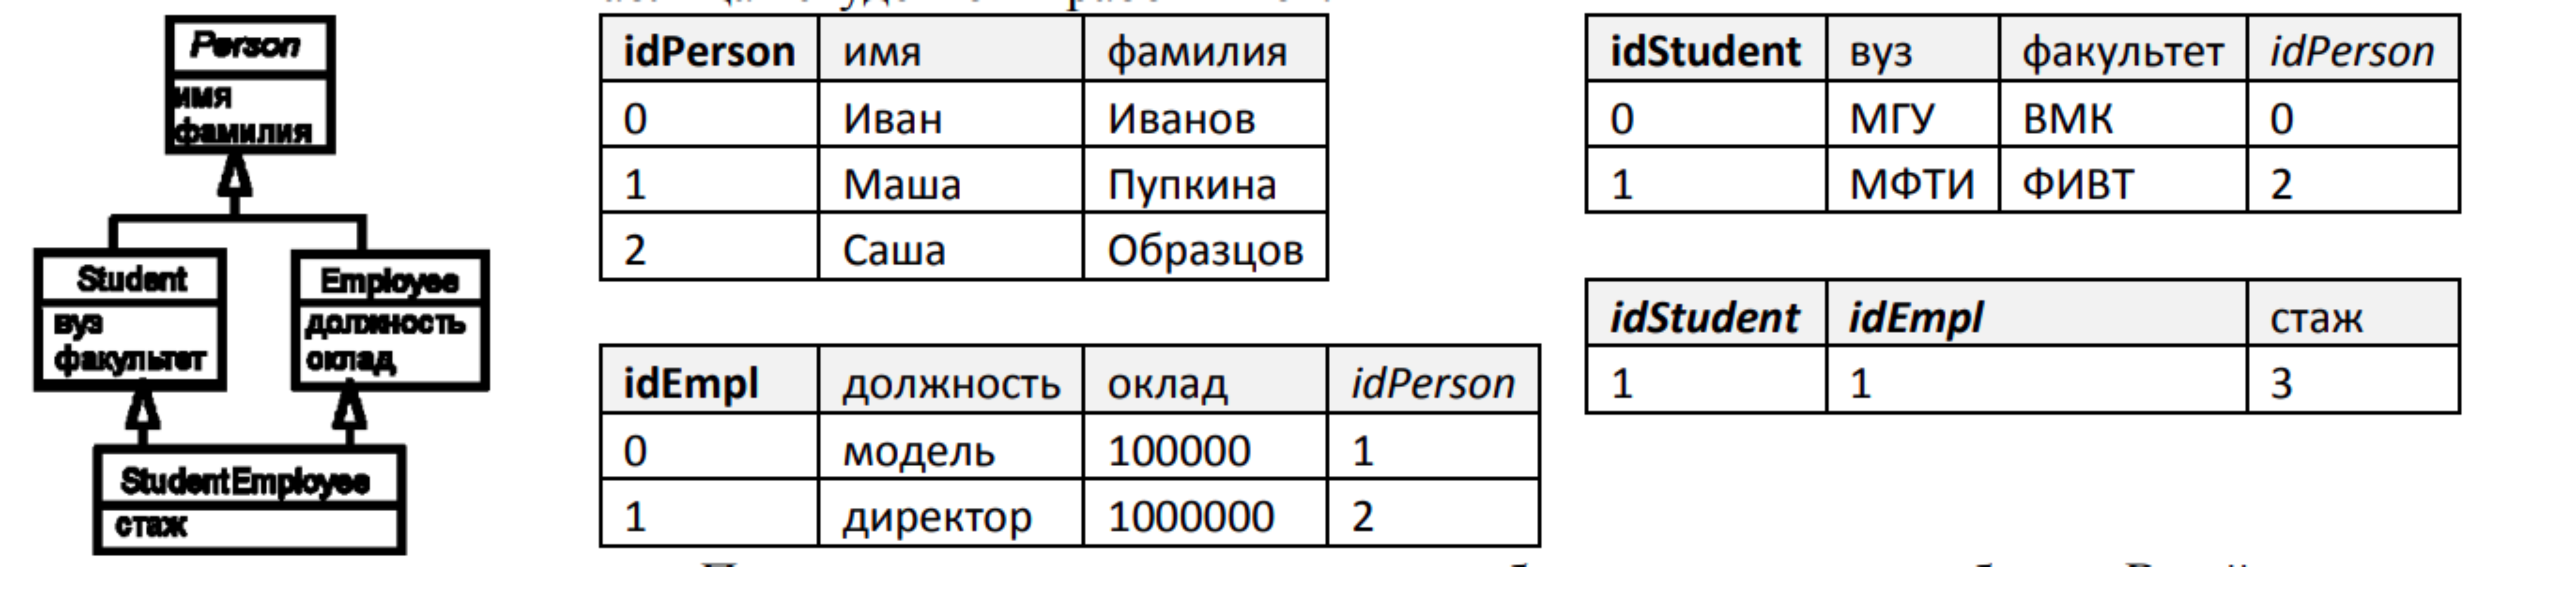
\includegraphics[scale=0.05]{pics/4_3.png}

\textbf{Стратегии}:

1) для каждого класса своя таблица (на картинке справа);

2) для всей иерархии наследования одна таблица (все поля в одной таблицы, добавятся в ней булевские isStudent и isEmployee, но будут пустые поля, например, не все обладают стажем);

3) таблицы только для конкретных (не абстрактных) классов (Person мы убираем, а поля имя и фамилия храним в Student и Employee);

4) таблицы только для различных конкретных классов (две таблицы: Student и Employee, в каждой стаж, в первой флаг isEmployee, во второй-isStudent).

Перейдём к тому, как с помощью диаграмм классов можно моделировать схемы БД. «pk, fk» (столбец, входящий в первичный и во внешний ключ помечается двумя стереотипами). Связи между таблицами моделируются как ассоциации между классами. Связь является идентифицирующей, если первичный ключ связанной таблицы включает в себя её внешний ключ, иначе не идентифицирующая. Для отображения ограничений целостности связь может моделироваться композицией. С её помощью описывается тот факт, что связанные записи одной таблицы следует удалить при удалении записи из другой таблицы («\textbf{черный закрашенный ромбик на схеме}»). Рассмотрим примеры из модели системы обработки заказов. Диаграмма с устойчивыми классами приведена ниже (и как мы её преобразовали в схему БД, нижняя схема, добавили табл со стат. атрибутами, +убрали выводимые атр., +табл TablePhone)
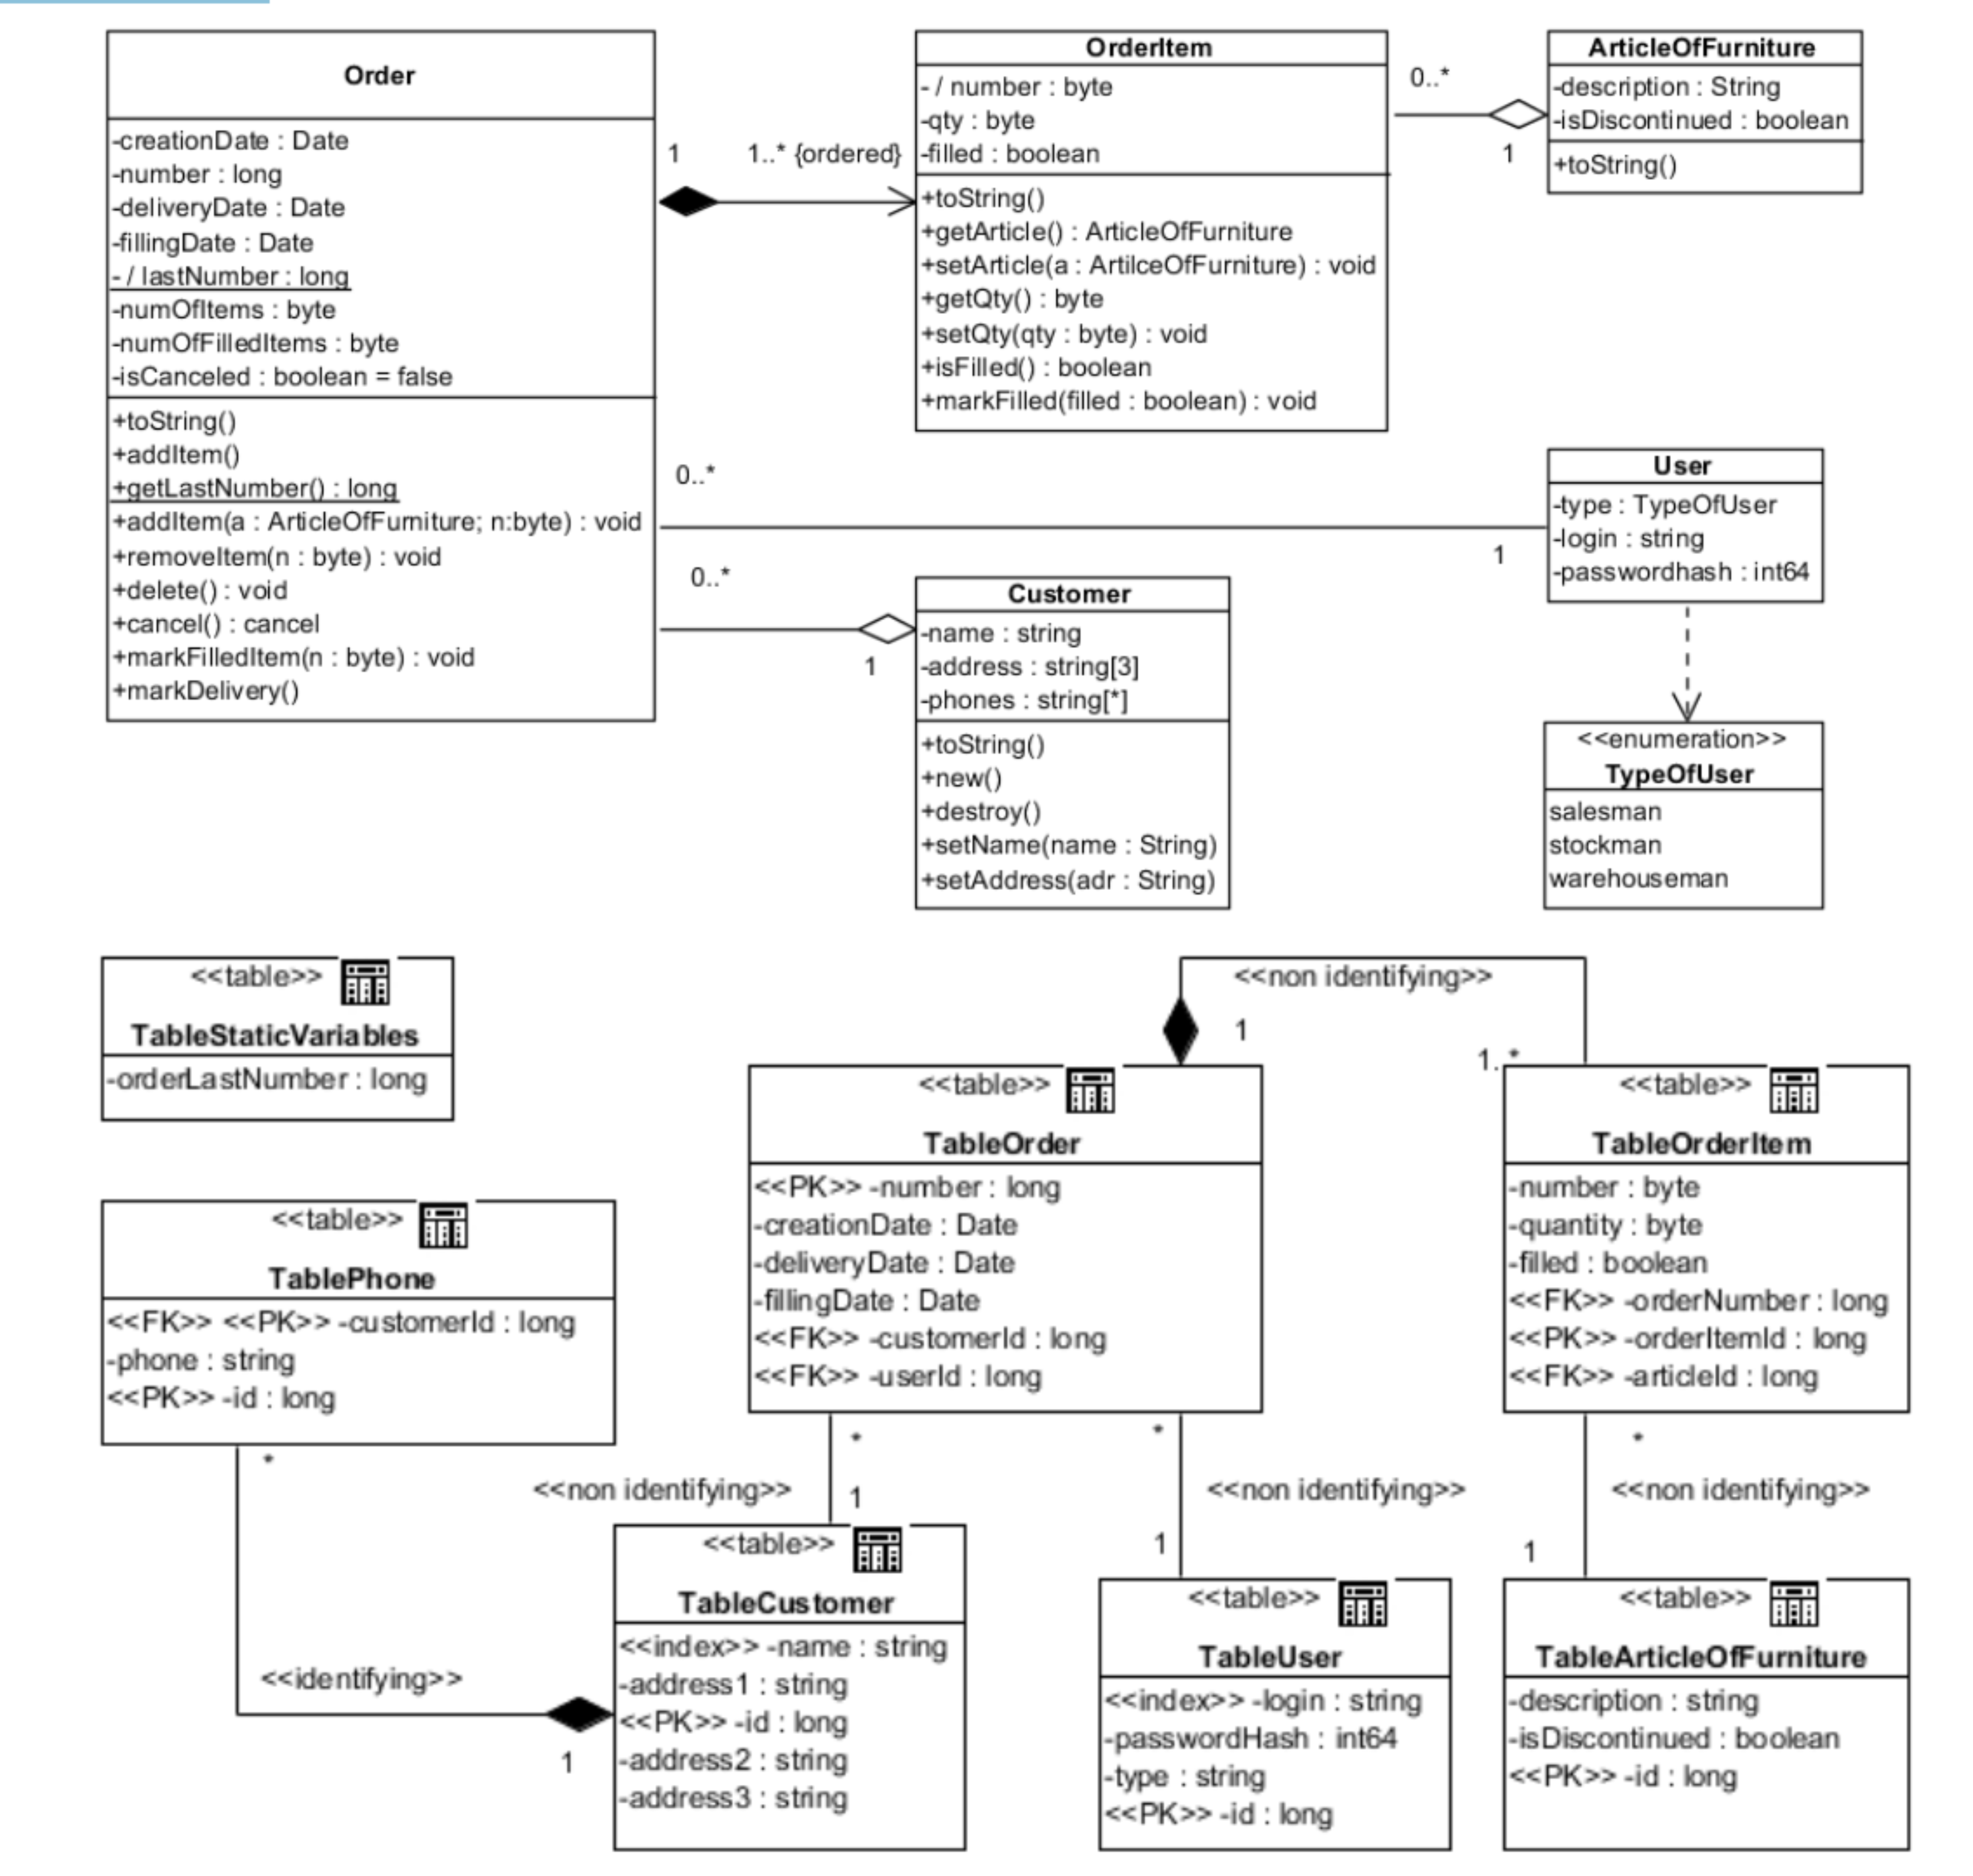
\includegraphics[scale=0.06]{pics/4_4.png}


\vfill\null
\columnbreak
%---------------------3--------------------
\subsection{OSN 2 Основные понятия дедуктивной верификации. Методы доказательства
завершимости программ.}

\vfill\null
\columnbreak
%---------------------
\end{multicols}
\end{tcolorbox}
% --- END OF PAGE ----



% --- BEGIN OF PAGE ----
\newpage  
\begin{tcolorbox}[colback=white, left=0mm, right=0mm]
\begin{multicols}{4}
%---------------------0--------------------
\subsection{OSN 9 Применение отладки для оценки возможности эксплуатации уязвимостей. Технологии отладки. Отладка пользовательского кода. Полносистемная отладка ввиртуальной машине. Статическое и динамическое инструментирование. Фаззинг. Разновидности фаззинга: черный ящик, белый ящик, серый ящик.}

\vfill\null
\columnbreak
%---------------------1--------------------
\subsection{OSN 11 Критерииполнотытестирования.Доменные,функциональные,структурныеи
проблемные критерии полноты. Использование графов, грамматик
илогических выражений для построения критериев полноты
тестирования.Типовыекритериипокрытия кода}

\vfill\null
\columnbreak
%---------------------2--------------------
\subsection{OSN 13 Интегрированные подходы построения тестов. Элементы технологии UniTESK.Программные контракты. Уточнение и формализация требований. Построение сценария теста на основе требований и заданного критерия полноты тестирования. Архитектура тестового набора UniTESK. Организация тестирования распределенных систем. Семантика чередования. Событийные контракты.}


\vfill\null
\columnbreak
%---------------------3--------------------
\nsection{OSN 15 Абстрактные модели: ошибки первого и второго родов (false positives, false negatives). Предикатная абстракция программ и уточнение абстракции по контрпримерам (CEGAR). Ее использование для верификации программ на языках программирования.}

2) смотри сюда: \url{http://sp.cmc.msu.ru/courses/vmp/kamkin_mc2018.pdf}, 
Страничка 173

\paragraph{}
Семантика LTL определяется на траекториях \textbf{структур Крипке}, т.е. на бесконечных последовательностях пометок -- \textit{множеств истинных элементарных высказываний}.

\paragraph{}
В вычислениях программ таких пометок нет, однако никто не мешает ввести высказывания о состояниях программы и использовать их для выражения требований. 
Например, если в программе есть переменные x и y,
можно определить высказывание (предикат) $p \equiv (x > y)$ и, <<измерив>> его истинность на всех состояниях некоторого вычисления проверить свойство $\textbf{G} \neg p$ (никогда значение переменной y не превосходит значения переменной x).

\paragraph{}
Для формальной верификации интерес представляют не одиночные траектории, а \textbf{все возможные траектории}. 
Для их представления нужно по программе построить ее модель в форме структуры Крипке.

\textbf{Структурой Крипке} называется четверка $\langle S, S_0, R, L \rangle$, где S -- множество \textit{состояний}, $S_0 \subseteq S$ -- множество \textit{начальных состояний}, $R \subseteq S \times S$ -- отношение переходов, $L:S \rightarrow 2^{AP}$ -- \textit{функция разметки}, помечающая каждое состояние структуры множеством истинных в нем элементарных высказываний (AP) (с помощью функции разметки задается интерпретация состояний).

Подробнее про структуры Крипке: страничка 144

\paragraph{}

\textit{Состояние}, или \textit{конфигурация}, является естественной концепцией, используемой в программировании. 
Это <<мгновенный снимок>> исполнения программы, включающий состояние данных (значения переменных) и состояние управления (точки исполнения процессов).

Пренебрегая некоторыми деталями, состояния можно объединять в классы эквивалентности, называемые абстрактными состояниями. 
Формализуем эту идею применительно к структурам Крипке:

Пусть заданы множество элементарных высказываний AP и структура Крипке $\langle S, S_0, R, L \rangle$, которую мы будем называть конкретной \textit{системой переходов}. 
Пусть $\hat{S}$  -- некоторое непустое множество -- множество абстрактных состояний. 
\textbf{Функцией абстракции} называется отображение $f: S \rightarrow \hat{S}$, такое что для всех $s, s' \in S$ имеет место импликация:

\begin{equation}
	(f(s) = f(s')) \rightarrow (L(s) = L(s')).
\end{equation}

\textit{Абстрактной системой переходов}, порожденной функцией абстракции f, называется система $\langle  \hat{S},  \hat{S_0},  \hat{R},  \hat{L} \rangle$, где

\begin{displaymath}
  \hat{S_0} = \{f(s) | s \in S_0\}, \hat{R} = \{ (f(s), f(s')) | (s, s') \in R \}
\end{displaymath}
  и
\begin{displaymath}
  \hat{L} (f(s)) = L(s) 
\end{displaymath}
для всех $s \in S$

\indent
\newline
Появление дополнительных траекторий в абстрактных моделях может привести к \textit{ложным сообщениям об ошибках} (\textit{false positives}), или, как их называют в математической статистике, \textbf{ошибкам первого рода}.

Для каждого найденного примера ошибочного поведения, так называемого \textit{контрпримера}, нужно проверить, \textit{реализуем ли он в исходной модели}: если нет, это не ошибка. 
Безусловно, ложные тревоги доставляют неприятности при анализе моделей, но гораздо более опасны \textbf{пропуски ошибок} (\textit{false negatives}) -- \textbf{ошибки второго рода}.

Если ошибки первого рода допустимы, то ошибки второго рода неприемлемы ни при каких обстоятельствах. 
Будем называть модель \textit{адекватной}, если она не допускает ошибок второго рода, а ее анализ требует привлечения приемлемых ресурсов (включая затраты на разбор ошибок первого рода).

\paragraph{Примечание снизу учебника:}
Ошибки \textbf{первого} и \textbf{второго} родов -- ключевые понятия проверки статистических гипотез. 
Ошибка \textbf{первого рода} -- нулевая гипотеза (например, гипотеза <<в программе нет ошибок>>) \textbf{неверно отвергнута}; ошибка \textbf{второго рода} -- нулевая гипотеза \textbf{неверно принята}.

\paragraph{Предикатные абстракции}

Пусть p -- предикат, заданный на множестве состояний S. Обозначим множество состояний, в которых предикат p истинен, как $[[p]]$, т.е. $[[p]] = \{s \in S | s \models p\}$.
Введем специальные предикаты \textit{false} и \textit{true}:
\begin{displaymath}
	[[false]] = \emptyset 
\end{displaymath}
и 
\begin{displaymath}
	[[true]] = S
\end{displaymath}

Пусть задано конечное множество предикатов $\{p_1, ..., p_n\}$.
Регионом называется предикат вида $\wedge^{m}_{k=1} p_{i_k}$, где $1 \leq i_1 < ... < i_m \leq n$, либо \textit{false}.
Если $m = 0$ то регион совпадает с \textit{true} (очевидно из формулы лол).

\paragraph{}
Метод абстракции, состоящий в «замене» конкретных состояний программы на формулы, описывающие множества состояний, называется \textbf{предикатной абстракцией}. 

Если формулы имеют вид \textit{регионов} (для некоторого заданного множества предикатов), метод называется \textbf{\textit{декартовой} предикатной абстракцией}.

\paragraph{CEGAR}

Метод CEGAR (\textit{Counter Example Guided Abstraction Refinement}) применяется для проверки достижимости определенной точки программы. Основная идея состоит в следующем:


Проверяется модель программы: если анализ выявляет, что модель корректна (заданная точка недостижима), то корректна и исходная программа (ошибки второго рода исключены); 
в противном случае для модели строится контрпример -- путь в заданную точку: если этот путь реализуем и в исходной программе, программа некорректна; 
иначе негативный результат проверки есть всего лишь ложная тревога, являющаяся следствием абстрагирования от чего-то существенного.
От чего именно, выявляется путем анализа контрпримера; модель уточняется, и к ней применяется тот же алгоритм. 
В результате ряда итераций метод CEGAR либо найдет путь в заданную точку, либо докажет ее недостижимость, либо, есть и такая возможность, упрется в ограничения по ресурсам.

\paragraph{Общая схема работы (формализованно):}

\begin{enumerate}
	\item Текущее множество предикатов полагается пустым. (два региона: $true$ и $false$)
			\begin{itemize}
				\item WHILE TRUE:
			\end{itemize}
	\item Строится абстрактная модель программы для текущего множества предикатов (для P).
	\item Проверяется корректность абстрактной модели (недостижимость точки $\textit{error}$):
		\begin{itemize}
			\item Если модель корректна, корректна и исходная программа, если нет -- идем дальше.
		\end{itemize}
	\item Строится контрпример $\pi$ -- вычисление из начальной конфигурации в конфигурацию вида $\langle \textit{error}, r \rangle$, где r -- регион, отличный от $\textit{false}$. \newline Конструируется сильнейшее постусловие $sp(op(\pi), \textit{true})$, где $\textit{op}(\pi)$ -- цепочка операторов SSA-представления, соответствующая вычислению $\pi$.
	\item Проверяется выполнимость формулы $sp(op(\pi), \textit{true})$:
		\begin{itemize}
			\item Если формула выполнима (SAT), исходная программа некорректна и $\pi$ -- контрпример. Если невыполнима (UNSAT) -- идем дальше.
		\end{itemize}
	\item Уточняется текущее множество предикатов: во множество добавляются предикаты, построенные на основе цепочки операторов $\textit{op}(\pi)$. \newline Осуществляется переход к шагу 2. \newline Заканчиваем, когда рассмотрели полное множество предикатов P и получили либо SAT в конкретном случае (тогда программа некорректна) или UNSAT во всех остальных случаях -- тогда не получилось построить контрпример (нет пути из какого-либо множества предикатов, ведущих в ошибочное состояние $error$) и это означает, что программа работает корректно.
\end{enumerate}

Кому всё еще непонятно -- глядите вот сюды: \url{https://forge.ispras.ru/attachments/download/8824/06-modeling-and-abstraction.pdf}.
\vfill\null
\columnbreak
%---------------------
\end{multicols}
\end{tcolorbox}
% --- END OF PAGE ----


% --- BEGIN OF PAGE ----
\newpage  
\begin{tcolorbox}[colback=white, left=0mm, right=0mm]
\begin{multicols}{4}
%---------------------0--------------------
\subsection{OSN 16 Информационная безопасность. Шифрование данных.
Криптографическаястойкость. Симметричная криптография. Блочный шифр
(DES) и его режимы.Ассиметричные схемы (RSA и Диффи-Хеллмана). Код
аутентификации (MAC).Цифроваяподпись(DSA).}


\vfill\null
\columnbreak
%---------------------1--------------------
\subsection{OSN 14 Спецификация и верификация параллельных программ. Синхронная и асинхронная параллельность. Справедливость планировщика.
Темпоральная логика линейного времени (LTL). Проблема взаимного исключения процессов.}

\vfill\null
\columnbreak
%---------------------2--------------------
\nsection{OSN 12 Методы контроля качества ПО. Верификация и валидация. Виды верификации. Экспертиза. Статический и динамический анализ. Формальные методы верификации. Проверка моделей.}

\textbf{Методы контроля качества ПО} предназначены для проверки различных характеристик качества ПО и поиска различных дефектов, связанных с недостаточным качеством. Они обычно разделяются на верификацию и валидацию. Они обычно разделяются на верификацию и валидацию.

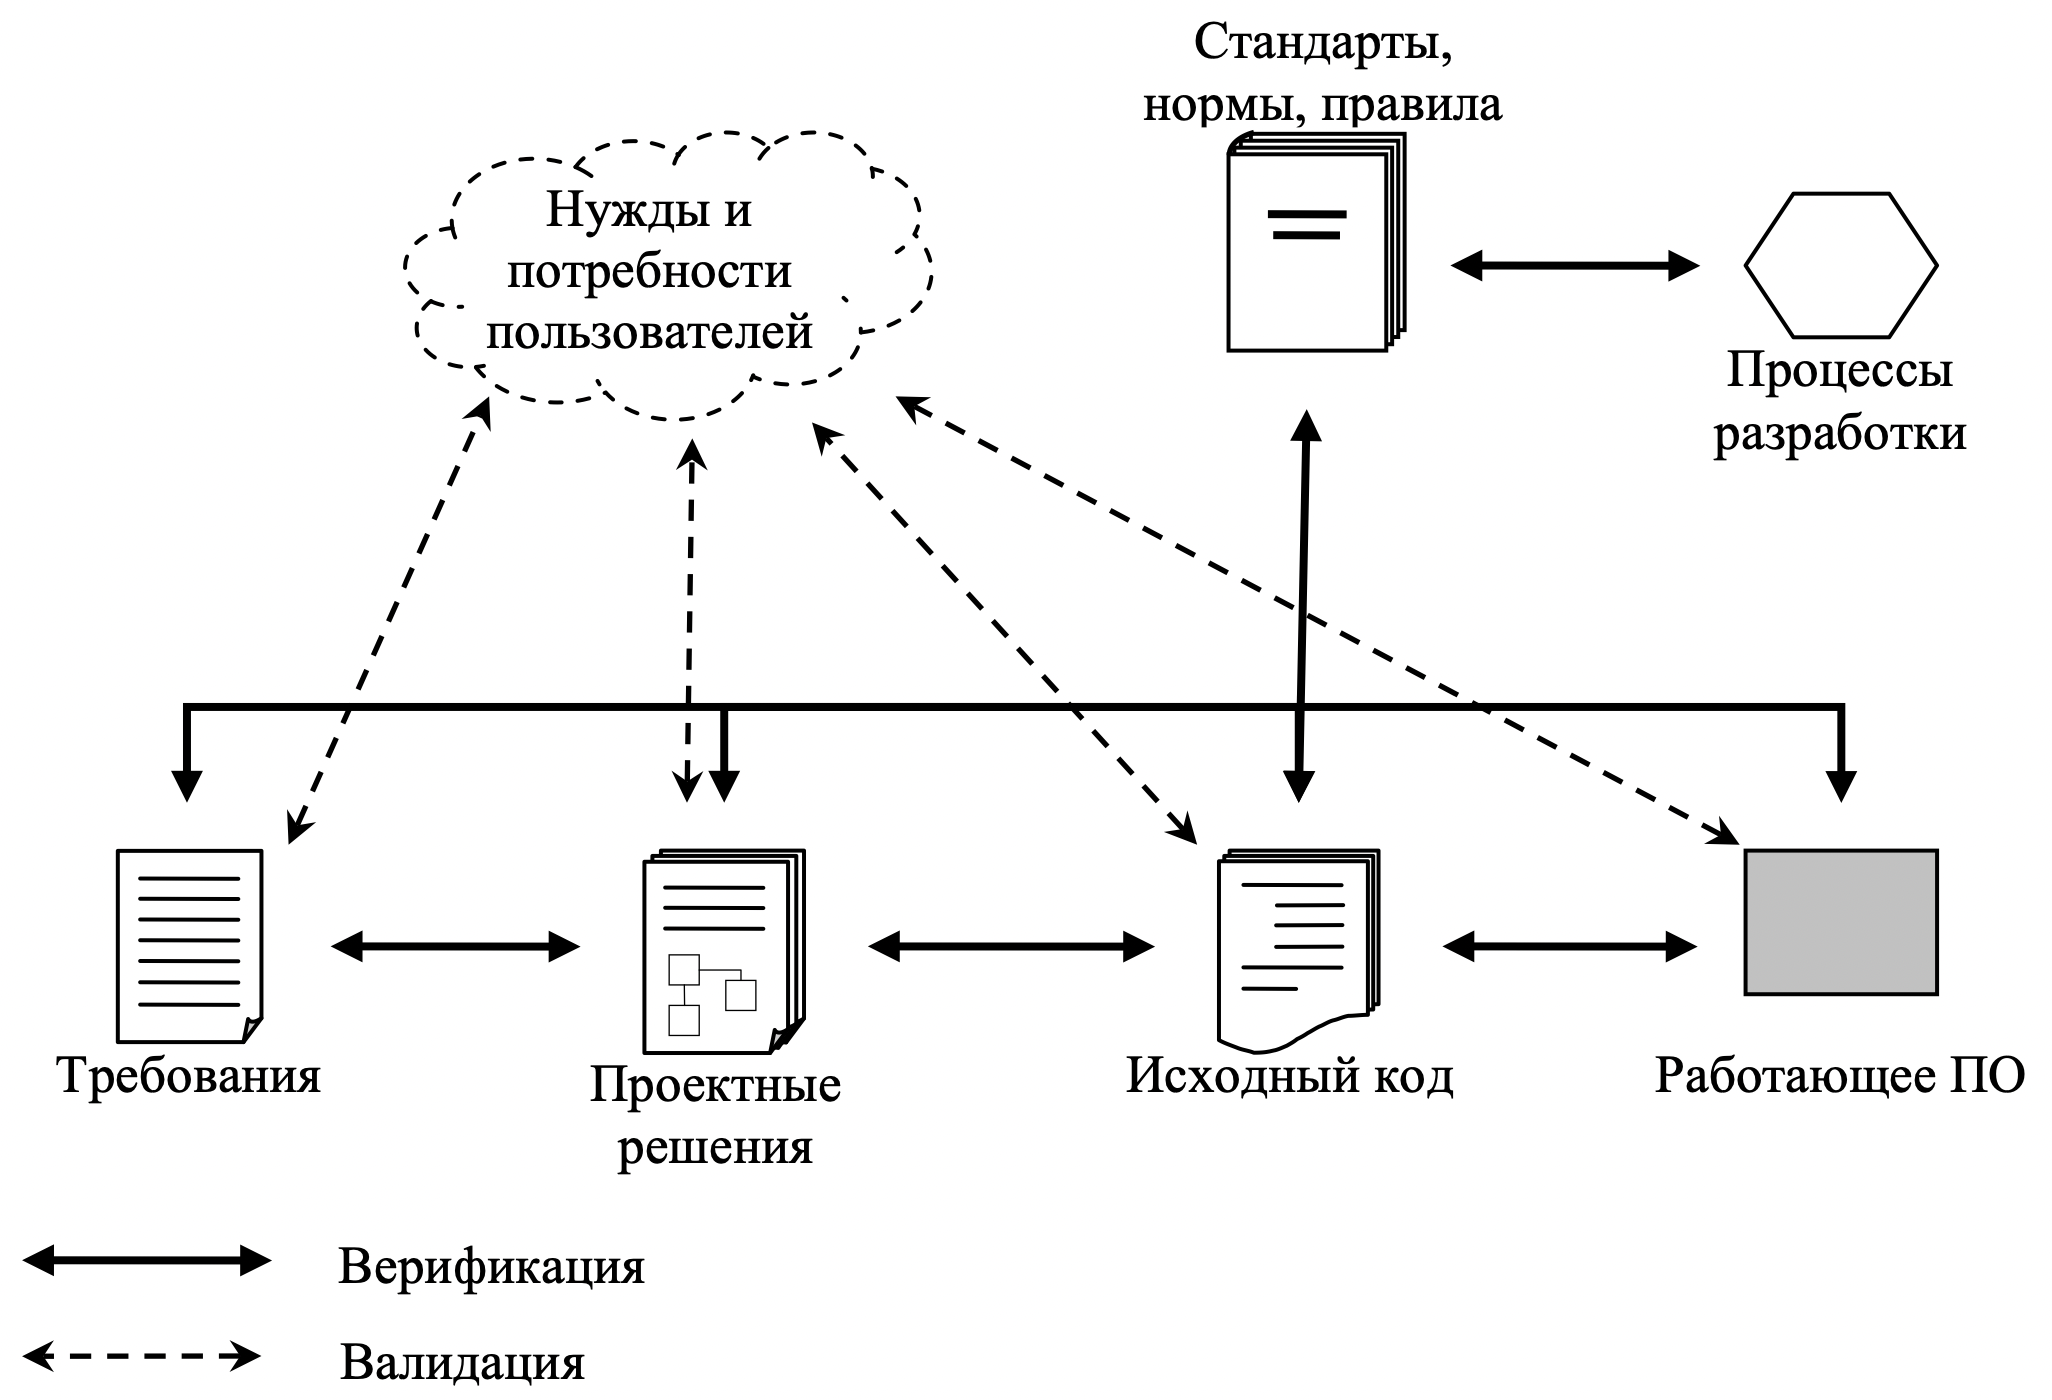
\includegraphics[scale=0.27]{pics/12_01.png}

\textbf{Валидация} обозначает проверку некоторого артефакта разработки на соответствие конечным целям, для достижения которых это ПО предназначено, т. е., нуждам и потребностям его пользователей и заказчиков. При валидации ПО проверяется, что оно действительно решает нужные пользователям задачи и удовлетворяет их потребности (даже если эти задачи и потребности описаны плохо и неполно). Валидация обычно проводится представителями заказчика, пользователями, экспертами в предметной области, т.е. людьми, обладающими достаточной компетентностью, чтобы судить о достижении поставленных целей. Если же эти цели формализовать, описать точно и полно, то проверка на соответствие полученному документу будет верификацией. Валидация необходима, потому что обычно согласованное, полное и точное описание задач сложной системы практически невозможно, разрабатываемые документы со спецификациями требований и пр. являются только приближениями к такому описанию. При валидации, могут использоваться те же техники, что и при выявления требований, поскольку цели этих видов деятельности похожи — преобразовать неясные и неформальные пожелания и представления о работе ПО в более точную форму (при валидации — в оценку проверяемых характеристик качества).

В рамках \textbf{верификации} качество некоторого артефакта (документа, модели, элемента кода и пр.) проверяется за счет сопоставления его с другим артефактом, на основе которого первый должен был быть разработан или которому он должен соответствовать (а также за счет проверки его соответсвия принятым нормам и стандартам разработки). Так, верифицировать код можно, имея на руках описание требований, проектные решения или стандарты кодирования, верифицировать проектный документ можно с помощью требований или стандартов на оформление подобных документов. Верифицировать можно и реальное поведение системы — сопоставляя его с требованиями, проектными решениями, принятыми стандартами функционирования систем такого рода. Методы верификации делятся на следующие группы:

\underline{\textit{1. Методы экспертизы}}. При экспертизе верификацию проводит человек, обладающий значительным опытом проведения такого рода проверок (часто также в экспертизу включаются неопытные сотрудники с целью их обучения). Экспертиза бывает общей, нацеленной на выявление любых дефектов и ошибок, или специализированной, направленной на оценку отдельных характеристик качества (например, гибкости архитектуры, удобства использования или защищенности ПО). Обычно в качестве видов экспертиз выделяют организационные экспертизы, технические экспертизы, сквозной контроль, инспекции и аудиты. Экспертиза применима к любым свойствам ПО и любым артефактам жизненного цикла и на любом этапе проекта, хотя для разных целей могут использоваться разные ее виды. Она позволяет выявлять практически любые виды ошибок, причем делать это на этапе подготовки соответствующего артефакта, тем самым минимизируя время существования дефекта и его последствия для качества итогового продукта. В то же время экспертиза весьма трудоемка, требует активного участия опытных людей и не может быть автоматизирована. Эффективность экспертизы существенно зависит от опыта и мотивации ее участников, организации процесса, а также от обеспечения корректного взаимодействия между различными участниками. Это накладывает дополнительные ограничения на распределение ресурсов в проекте и может приводить к конфликтам между разработчиками, если руководство проекта обращает мало внимания на коммуникативные аспекты проведения экспертиз.

\underline{\textit{2. Статический анализ}}. Такие методы используют автоматический анализ кода, моделей или других документов разработки с целью проверки выполнения формализованных правил их оформления (синтаксической корректности) и поиска часто встречающихся ошибок по определенным шаблонам (разыменования нулевых указателей, обращения к неинициализированным данным, деления на 0, взаимной блокировки параллельных процессов и пр.).
Статический анализ выполняется с помощью специализированных инструментов, техники статического анализа кода, которые достигли достаточной зрелости и поддерживаются эффективными алгоритмами, чаще всего включаются в состав компиляторов. Однако, статический анализ обычно способен выявлять лишь ограниченный набор видов ошибок.
Основной проблемой многих техник статического анализа является следующая дилемма: либо используются строгие методы анализа, не допускающие пропуска ошибок (тех типов, что ищутся), но приводящие к большому количеству сообщений о возможных ошибках, которые таковыми не являются (ложные сообщения об ошибках), либо набор сообщений об ошибках является точным, но возникает возможность пропустить ошибку. Обычно используются компромиссные решения, позволяющие обнаруживатькак можно больше ошибок, но допускающие не слишком высокий процент ложных сообщений.

\underline{\textit{3. Динамический анализ}}. Эти методы выполняют верификацию реальной работы ПО или работы его кода или исполнимой модели (из которой код получают автоматизированной трансляцией) в специализированном окружении (например, при отсутствии нужного оборудования или внешних систем производится их эмуляция). При этом собирается информация о результатах работы в различных ситуациях, и эта информация далее подвергается анализу на предмет соответсвия требованиям или проектным решениям. Обычно к таким методам относят тестирование, при котором работа ПО проверяется на заранее выбранном наборе ситуаций; мониторинг, в рамках которого работа ПО протоколируется и оценивается при его обычной или пробной эксплуатации; а также профилирование, специфический вид мониторинга временных характеристики работы ПО и использования им отдельных ресурсов. К динамическим методам анализа относят также и имитационное тестирование и имитационный мониторинг, при которых ПО выполняется в рамках какого-то модельного окружения, построенного с использованием симуляторов и эмуляторов. Для применения динамических методов необходимо иметь работающую систему или хотя бы некоторые ее компоненты, или же их прототипы, поэтому нельзя использовать их на первых стадиях разработки.

\underline{\textit{4. Формальные методы верификации}} используют формальные математические модели проверяемого артефакта и того, на соответствие которому проводится проверка. Чаще всего это модели, соответственно, кода или проектных решений и требований. К формальным методам относятся дедуктивный анализ и проверка моделей. В рамках дедуктивного анализа свойства кода или проектных решений, а также требования формализуются в виде наборов логических утверждений (могущих включать элементы логики высших порядков и различных алгебраических структур), и из первого набора I (решения) пытаются формально вывести второй S
(требования), т.е., пытаются строго доказать выводимость I $\vdash$ S. \textbf{Проверка моделей} основана на представлении проверяемых решений в виде автоматных моделей M, а требований к ним — в виде наборов логических утверждений S (обычно с элементами временной или модальной логики). Далее выполняется автоматическая проверка
выполнения M $\models$ S этих утверждений на полученных моделях с помощью специализированных инструментов. При этом обнаруживаемые ошибки могут быть сразу же оформлены как контрпримеры, конкретные сценарии работы проверяемой модели, при которых сформулированные требования нарушаются.

Формальные методы применимы только к тем свойствам, которые выражены в рамках некоторой математической модели, а также к тем артефактам, для которых можно построить адекватную формальную модель. Для использования таких методов необходимо затратить значительные усилия на построение формальных моделей. К тому же, построить такие модели и провести их анализ могут только специалисты по формальным методам, которых не так много, и чьи услуги стоят достаточно дорого. Построение формальных моделей нельзя автоматизировать, для этого всегда необходим человек. Анализ их свойств в значительной мере может быть автоматизирован, и сейчас уже есть инструменты, способные анализировать формальные модели промышленного уровня сложности, однако чтобы эффективно пользоваться ими часто тоже требуется очень специфический набор навыков и знаний (в специфических разделах математической логики и алгебры).

% Взято из: https://mbt-course.narod.ru
% лекция 1
\vfill\null
\columnbreak
%---------------------3--------------------
\subsection{OSN 10 Символьное выполнение: основные понятия. Схема работы системы
символьного выполнения. Предикат пути, предикат безопасности. Проблема
экспоненциального взрыва, стратегии выбора следующего состояния.}

\vfill\null
\columnbreak
%---------------------
\end{multicols}
\end{tcolorbox}
% --- END OF PAGE ----



% --- BEGIN OF PAGE ----
\newpage  
\begin{tcolorbox}[colback=white, left=0mm, right=0mm]
\begin{multicols}{4}
%---------------------0--------------------
\nsection{OSN 17 Понятие анонимности пользователя в сети. Идентификаторы пользователя в сети на разных уровнях (устройства, ОС, ПО). Подходы к деанонимизациии, способы защиты. Концепция анонимных сетей (Mix и Tor). Луковая маршрутизация. Виды атак на анонимные сети.}

\subsubsection{Анонимность пользователя в сети}

\begin{itemize}
    \item Защита от наблюдения со стороны Интернет-провайдера (а также тех, кто его контролирует):
    – цензура
    
    – контекстная реклама
    
    – осуществление общественной, гражданской или политической деятельности
    \item Защита от наблюдения со стороны посещаемого ресурса    
\end{itemize}

\begin{itemize}
    \item Социальная анонимность – распространение (осознанное/неосознанное) в сети
персональной информации самим пользователем
    \item Техническая анонимность:
    
    – контроль за хранением и безопасностью персональных данных посредством специальных технических средств (как программных, так и аппаратных)
    
    – минимизация возможности утечки персональных данных
\end{itemize}

\textbf{Анонимность субъекта} (anonymity) -- злоумышленник не может с достаточной степенью точности идентифицировать субъект в рамках некоторого множества субъектов со схожим
набором атрибутов.

\textbf{Виды анонимности}:
\begin{itemize}
    \item Анонимность отправителя -- ни получатель сообщения, ни атакующий, наблюдающий за некоторым участком сети (между отправителем и получателем), не могут установить отправителя сообщения
    \item Анонимность получателя -- атакующий, наблюдающий за некоторым участком сети, не может установить получателя сообщения
    \item Анонимность взаимодействия -- атакующий, наблюдающий за некоторым участком сети, не может достоверно установить, от какого отправителя и какому получателю доставляется конкретное сообщение
    \item $K$-анонимность: пользователь сети не может на практике отличаться, по крайней мере, от $(K - 1)$ других пользователей сети, когда $K$ достаточно большое. Вводится для количественной оценки уровня анонимности, предоставляемого системой анонимизации отдельному пользователю
\end{itemize}

\subsubsection{Идентификаторы пользователя в сети}

Устройство пользователя:
\begin{itemize}
    \item \textit{Адресные признаки устройства}: MAC-адрес сетевого интерфейса, IP-адрес, назначенный сетевому интерфейсу
\end{itemize}

ПО пользователя:
\begin{itemize}
    \item \textit{Операционная система} (реализация стека протоколов TCP/IP): Windows 10, Ubuntu 20.04, iOS 13.2.2, ...
    \item \textit{Сетевое приложение}: User-Agent, Cookies, цифровой отпечаток, ...
\end{itemize}

\subsubsection{Подходы к деанонимизациии, способы защиты}

\textbf{Деанонимизирующие признаки ОС}: стек TCP/IP. Основаны на пробелах в
спецификациях протоколов, и, следовательно, различных реализациях в разных ОС:
\begin{itemize}
    \item IPv4: генерация значения поля ID при фрагментации, выбор начального значения TTL, установка флага DF для пакетов, не требующих фрагментации
    \item ICMP: Destination Port Unreachable, размер фрагмента не фиксирован
    \item TCP: выбор начального значения sequence number, ответы на некорректные комбинации флагов, набор опций (порядок передачи, поддержка)
\end{itemize}

Деанонимизация ОС:

\textbf{Активное сканирование:}

Злоумышленник формирует и отправляет сообщения с заданными свойствами, после чего анализирует полученные ответы. Обладает большей точностью. Может быть обнаружено системами обнаружения вторжений (IDS). Известный представитель: Nmap.

\textbf{Пассивное сканирование:}

Злоумышленник анализирует прослушиваемый трафик, ничего не отправляя в сеть. Является менее точным. Не может быть обнаружено – Известный представитель: p0f.

\textbf{Обеспечение технической анонимности}

Сокрытие факта взаимодействия между двумя узлами сети для некоторого потока сетевых пакетов:
\begin{itemize}
    \item Скрыть адресные признаки узла-отправителя и узла-получателя
    \item Скрыть идентификаторы уровня ОС
    \item Сделать цифровой отпечаток пользователя «стандартным»
\end{itemize}

Сокрытие адресных признаков: отказаться от прямой передачи данных от узла-отправителя к узлу-получателю
\begin{itemize}
    \item осуществлять передачу данных через один или несколько промежуточных узлов
\end{itemize}

\subsubsection{Концепция анонимных сетей (Mix и Tor)}

\begin{itemize}
    \item Обобщают подход на основе использования промежуточных узлов: используется цепочка из нескольких узлов
    \item Ни один промежуточный узел не знает одновременно адреса источника и адреса назначения, большинство промежуточных узлов не знает ни того, ни другого адреса
\end{itemize}

\textbf{Mix сети}:

Впервые предложены в 1981 году. Каждый узел знает только свою часть маршрута -- вложенное шифрование с использованием публичных ключей всех участвующих в передаче узлов, защита от отдельных скомпрометированных узлов. 

Mix-сети относятся к группе анонимных сетей с высокой задержкой – это ограничивает их применимость (ок для электронной почты, не ок для анонимного просмотра веб-страниц/видео).

Используется цепочка прокси-серверов, каждый из которых:

- получает сообщения от большого числа источников
    
- изменяет порядок отправки сообщений
    
- посылает в измененном порядке сообщения следующему прокси-серверу или получателю

\textbf{Tor}

Децентрализованная сеть, поддерживаемая добровольцами. Исходный код в открытом доступе. Считается одним из самых надежных способов обеспечения анонимности в сети Интернет.

Типы узлов:
\begin{itemize}
    \item \textbf{Входные узлы} -- принятие соединений, инициированных клиентами, их шифрование и перенаправление к следующему узлу
    \item \textbf{Узлы посредники} -- передача шифрованного трафика следующим узлам
    \item \textbf{Выходные узлы} -- передаточное звено между клиентом сети Tor и публичным Интернетом
    \item \textbf{Сторожевые узлы} -- клиент выбирает три узла в качестве сторожевых и использует один из них в качестве входного узла для каждой создаваемой цепочки
    \item \textbf{Мостовые узлы} входные узлы сети Tor, адреса которых не публикуются в сервере каталогов, а передаются только по запросу
    \item \textbf{Управляющие узлы} - распределены по миру, <<зашиты>> в ПО клиента, владеют информацией о состоянии всей Tor сети
\end{itemize}

\subsubsection{Луковая маршрутизация}

\begin{wrapfigure}[7]{r}{0.5\linewidth}
\vspace{-6.5ex}
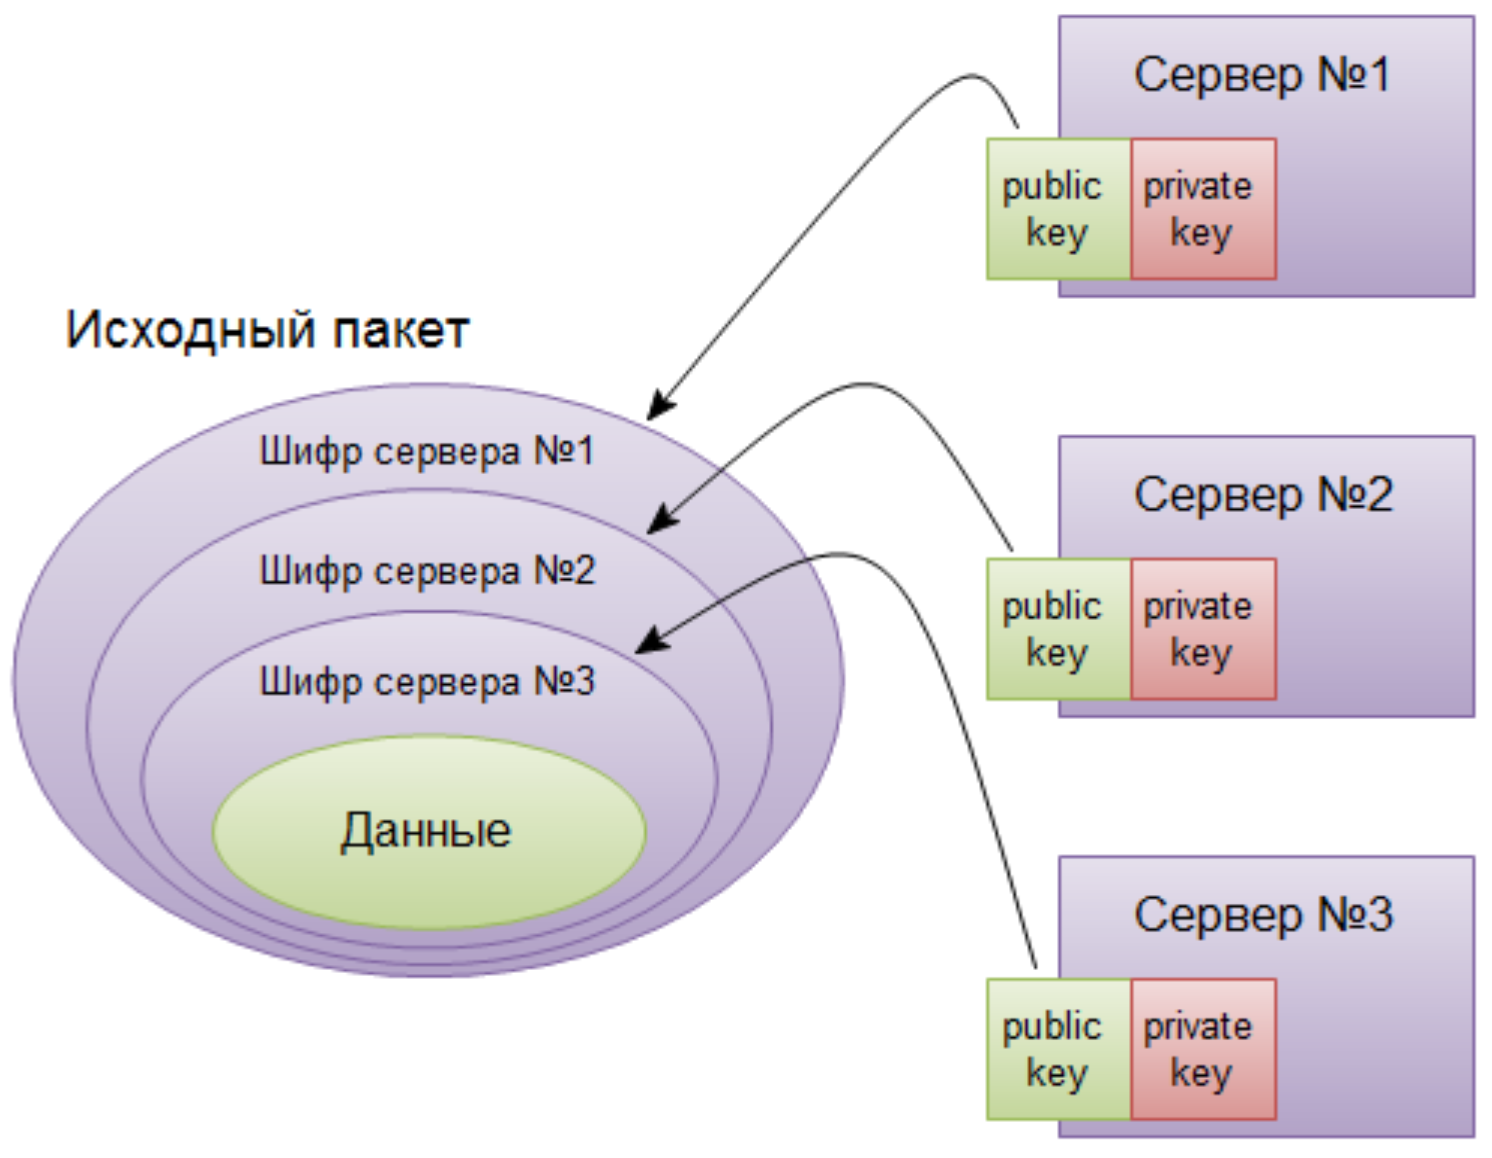
\includegraphics[scale=0.18]{pics/onion-routing.png}
\end{wrapfigure}

Каждый отдельный уровень шифрования дешифруется очередным маршрутизатором. Из дешифрованных данных извлекается адрес следующего маршрутизатора. Сообщение отправляется на следующий маршрутизатор.

\subsubsection{Виды атак на анонимные сети}

\begin{enumerate}
    \item \textit{Атака на кодировку сообщения}. Если сообщение не меняет свое содержимое при прохождении по анонимной сети, весь его маршрут может быть восстановлен
    \item \textit{Атака на длину сообщения}. Если сообщение сохраняет свой размер при передаче по сети, его маршрут может быть восстановлен
    \item \textit{Атака на воспроизведение}. Атакующий может воспроизводить данные ранее переданных сообщений, ожидая, что сеть передаст эти пакеты по тому же маршруту
    \item \textit{Атака путем сговора}. Некоторые участники анонимной сети объединяются для нарушения анонимности остальных участников
    \item \textit{Атака на переполнение}. Переполнение отдельных каналы анонимной сети, чтобы сузить круг пользователей, к которым эти сообщения могут относиться
    \item \textit{Временные атаки}. Оценка продолжительности соединения путем наблюдения фактов установки и окончания соединения в различных точках входа и выхода сети
    \item \textit{Атака на объем данных}. Сопоставление общего объема передаваемых данных в точках входа и выхода сети
    \item \textit{Атака профилирования}. Долговременный анализ соединений некоторого набора пользователей -- обычно комбинация временных атак и атак на объем данных
\end{enumerate}

\vfill\null
\columnbreak

\end{multicols}
\end{tcolorbox}
% --- END OF PAGE ----


% --- BEGIN OF ADDITIONAL PAGE ----
\newpage  
\printbibliography
% --- END OF ADDITIONAL PAGE ---


\end{document}
